
\chapter{Literature Review}
\label{ch:chapter2}

\begin{figure}[H]
	\centering
	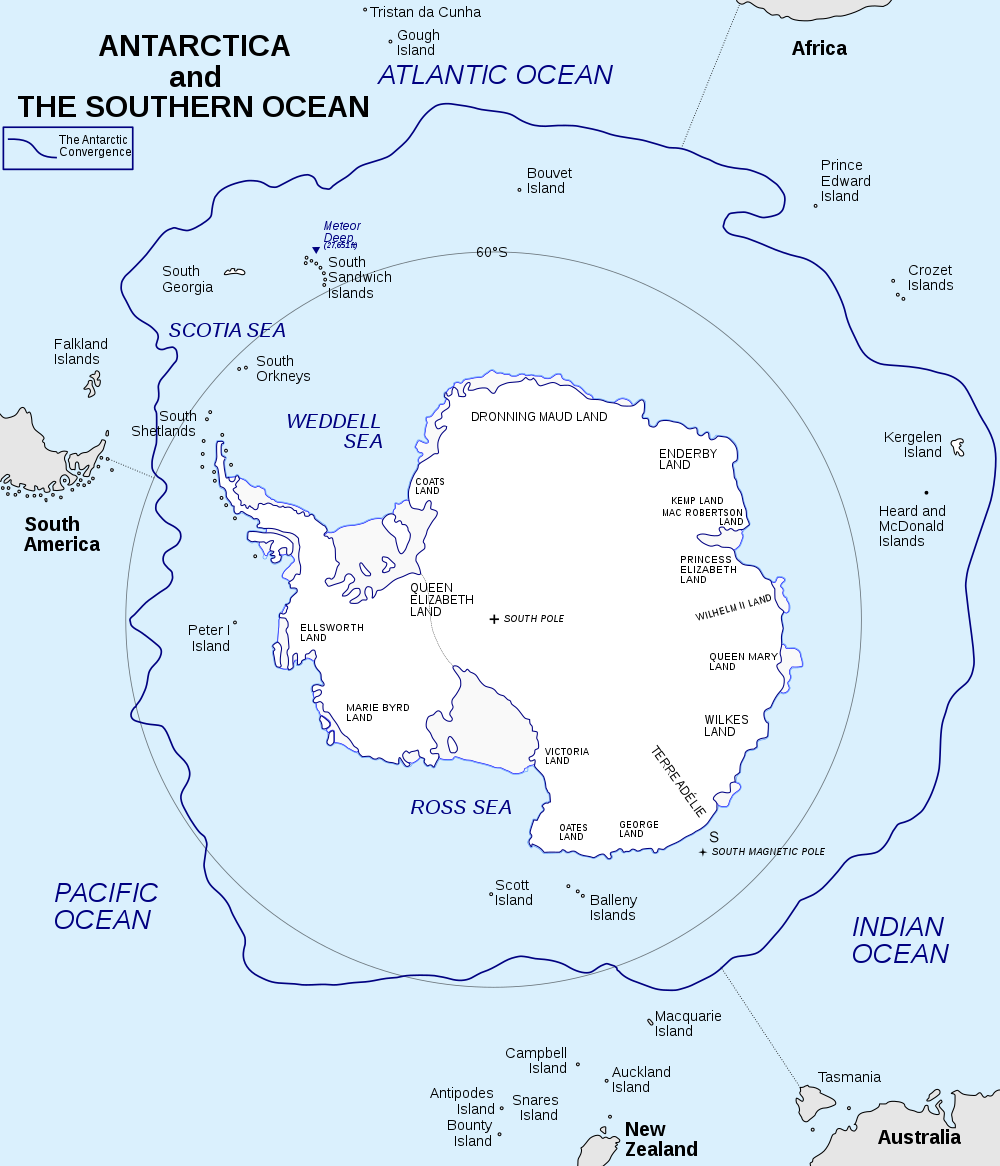
\includegraphics[width = 10cm,height=10cm]{Antarctica_and_the_Southern_Ocean.png}
	\caption{Map of the Southern Ocean surrounding the Antarctic continent. Image created by \textcite{Hogweed2015Ocean} and licensed by CC BY-SA 3.0}
	\label{fig:Antarctica_Southern_Ocean}
\end{figure}

As highlighted by section \ref{sec:ch1.section1}, there is a great desire by research scientists for in situ instruments to provide observation data which fills spatial and temporal measurement gaps in Antarctic sea ice monitoring in the Southern Ocean as shown in figure \ref{fig:Antarctica_Southern_Ocean}. This chapter investigates the current use of autonomous monitoring technology used by research scientists in this region focusing on progress made to improving in situ observations and highlighting areas for improvement.
%%%%%%%%%%%%%%%%%%%%%%%%%%%%%%%%%%%%%%%%%%%%%%%%%%%%%%%%%%%%%%%%%%%%%%%%%%%

\newpage
\section{In situ climate sensing technologies}


\begin{figure}[H]
	\centering
	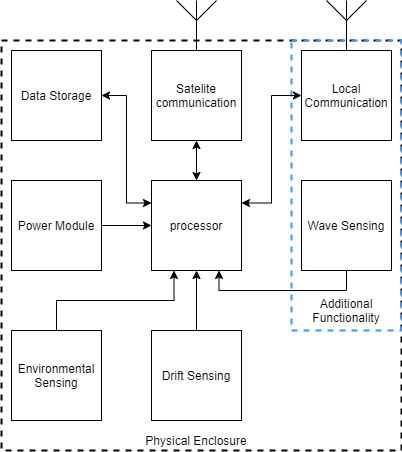
\includegraphics[width = 0.5\linewidth]{device block diagram.png}
	\caption{A block diagram of a typical device for in situ measurements. Each device contains modules for environmental sensing and drift sensing connected to a processor. This can be a micro-controller or microprocessor. Additionally, a data storage module (such as an SD card) is included to store data during the operation. Some device include modules for local communications or wave sensing units. Finally, a remote communication module is included to transfer the data to a research center or a user. The electronics are placed inside a physical enclosure for protection against the polar climate while a portable power module supplies the device during its operation.}
	\label{fig:devblockdiag}
\end{figure}

Autonomous instrumentation has seen increased use for in situ observations in the polar sea ice regions \cite{kennicutt2016delivering}. These devices have typically  been developed by the commercial sector \cite{rabault2017measurements} from companies such as Trident \cite{trident}, MetOcean \cite{uptempo}, Seabird \cite{seabird2021website} and Sea Technology Services (STS) \cite{sts2021website}. Additionally, academic institutions have also developed in situ measurement devices such as The University of Washington's SWIFT buoy \cite{thomson2012wave} or University of Dartmouth's Seasonal Ice Mass Balance (SIMB) buoy \cite{polashenski2011seasonal}. While these technologies have the benefit of reliability, they are often expensive \cite{rabault2017measurements} and inflexible to the specific needs of polar scientists. Technology has reached a point where low-cost and open source alternatives are well documented and reliable enough to be integrated into customized solutions \cite{rabault2019open}.\par 


In this section, a comparison of data collection devices used in the polar regions is presented as well as  description of their design, opperation and deployment. Where possible, certain specifications have been converted into standardised formats. To ensure a fair evaluation, data were collected from the latest technical publication of each platform where possible. These publications may not contain all relevant data. In this case, the data entry has been marked with a "Not reported" or "NR". Figure \ref{fig:buoys}.


Eight platforms were selected for the comparison with each device designed by a private company or an institution. The key collaborators as well as the name of the institution are provided in table \ref{tab:device_list}. Where a buoy name is not given, the device will be named after the key contributor to the project. These systems have been selected due to their prevalence in global polar/ oceanographic science as well as notability in publications. Device performance will be evaluated in the context of the requirements set out by \textcite{kennicutt2016delivering} for an autonomous in situ measurement device shown in section \ref{sec:ch1.section1}. 

\label{ch2:secdevice}
\begin{figure}[H]
	\centering
	\begin{subfigure}[b]{0.24\textwidth}
		\centering
		\begin{tikzpicture}
			\node[anchor=south west,inner sep=0] (image) at (0,0) { 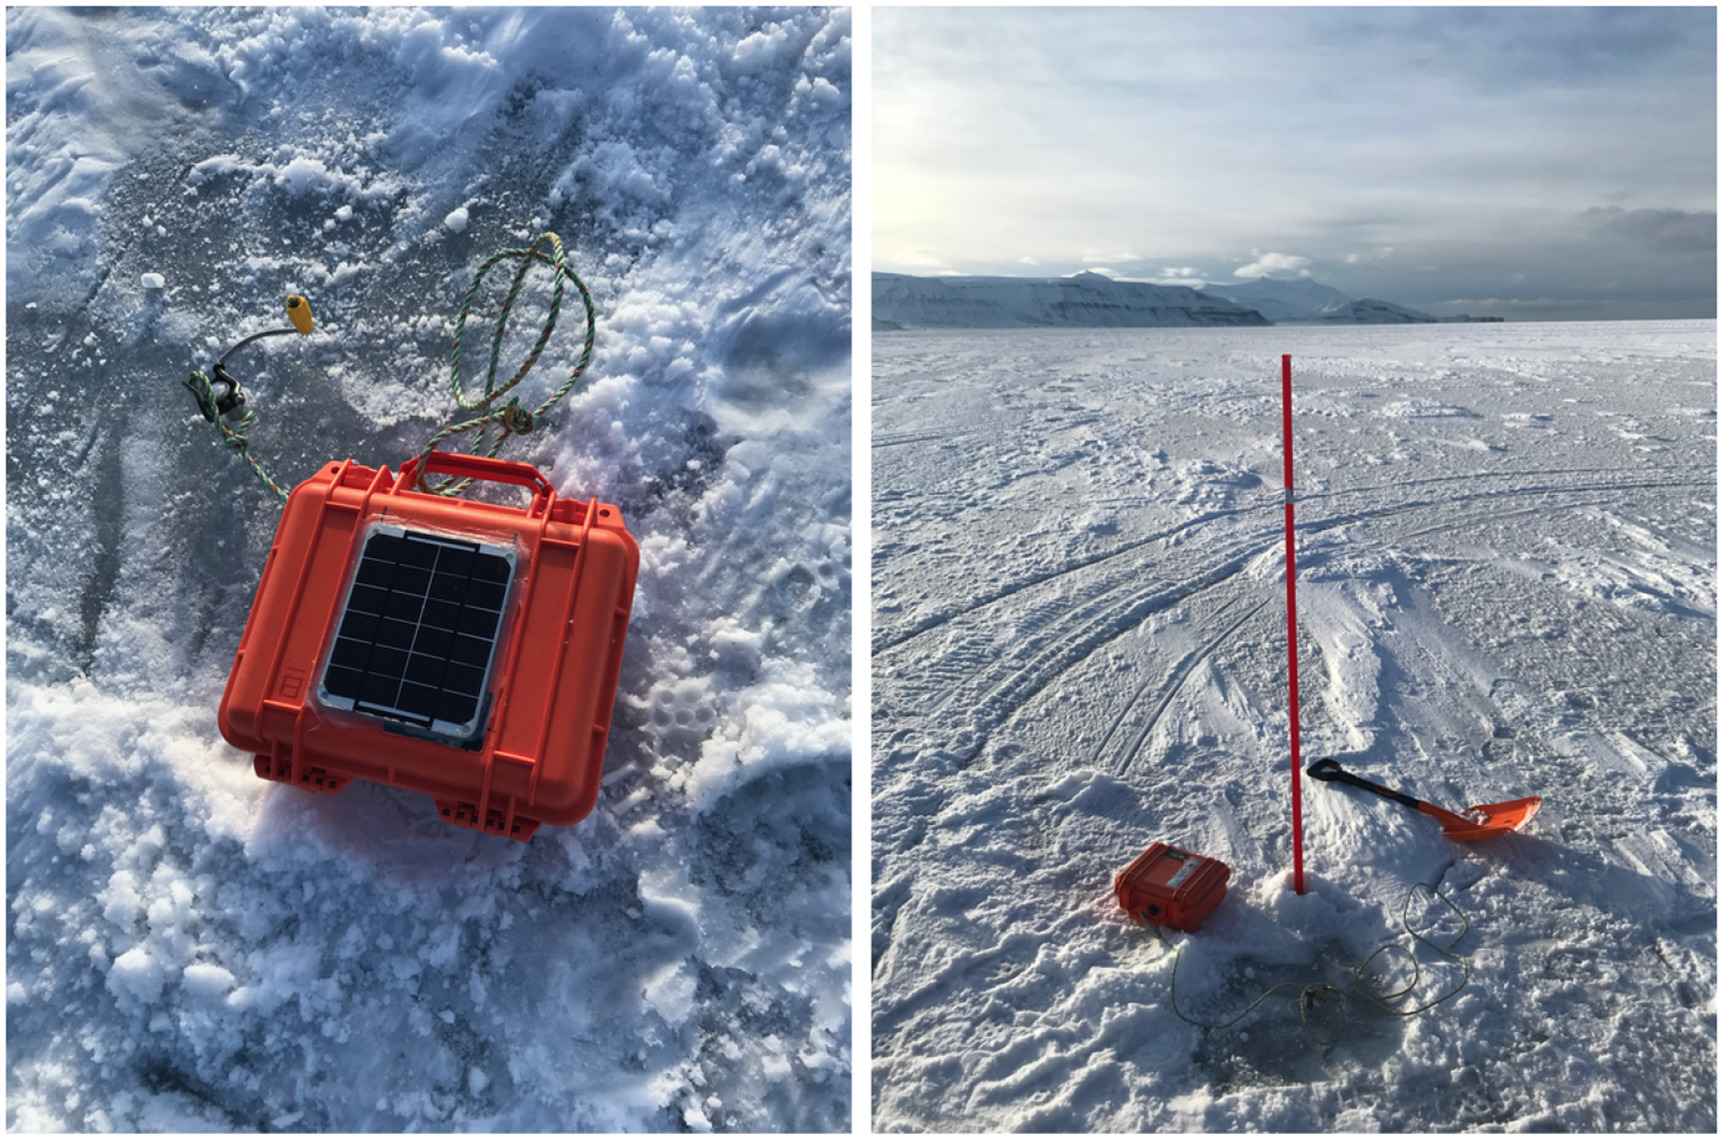
\includegraphics[width = 4cm,height=4cm]{WIIB.jpg}};
			\begin{scope}[x={(image.south east)},y={(image.north west)}]
				\draw[color=black, ultra thin,fill=white] (0.0,0.0) rectangle (0.21,0.16) node[pos=.5] {A};
			\end{scope}
		\end{tikzpicture}
		\label{fig:WIIB}
	\end{subfigure}%
	\hfill
	\begin{subfigure}[b]{0.24\textwidth}
		\centering
		\begin{tikzpicture}
			\node[anchor=south west,inner sep=0] (image) at (0,0) { 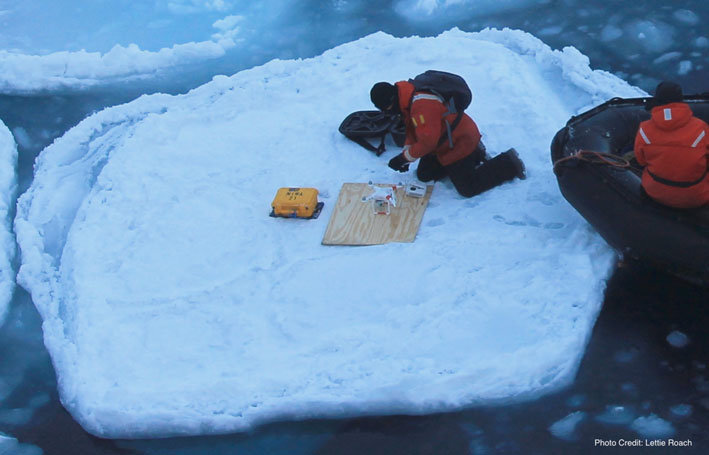
\includegraphics[width = 4cm,height=4cm]{WIIOS.png}};
			\begin{scope}[x={(image.south east)},y={(image.north west)}]
				\draw[color=black, ultra thin,fill=white] (0.0,0.0) rectangle (0.21,0.16) node[pos=.5] {B};
			\end{scope}
		\end{tikzpicture}
		\label{fig:WIIOS}
	\end{subfigure}%
	\hfill
	\begin{subfigure}[b]{0.24\textwidth}
		\centering
		\begin{tikzpicture}
			\node[anchor=south west,inner sep=0] (image) at (0,0) { 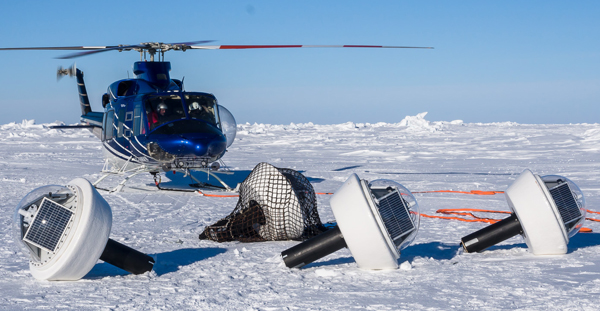
\includegraphics[width = 4cm,height=4cm]{doble.jpg}};
			\begin{scope}[x={(image.south east)},y={(image.north west)}]
				\draw[color=black, ultra thin,fill=white] (0.0,0.0) rectangle (0.21,0.16) node[pos=.5] {C};
			\end{scope}
		\end{tikzpicture}
		\label{fig:NDWB}
	\end{subfigure}%
	\hfill
	\begin{subfigure}[b]{0.24\textwidth}
		\centering
		\begin{tikzpicture}
			\node[anchor=south west,inner sep=0] (image) at (0,0) { 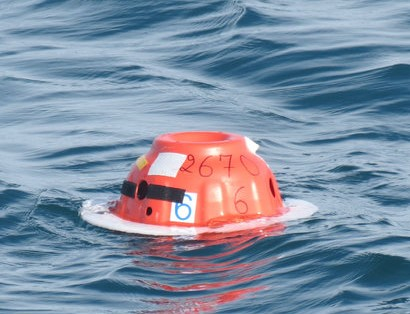
\includegraphics[width = 4cm,height=4cm]{SKIB.png}};
			\begin{scope}[x={(image.south east)},y={(image.north west)}]
				\draw[color=black, ultra thin,fill=white] (0.0,0.0) rectangle (0.21,0.16) node[pos=.5] {D};
			\end{scope}
		\end{tikzpicture}
		\label{fig:SKIB}
	\end{subfigure}%
	\hfill
	\begin{subfigure}[b]{0.24\textwidth}
		\centering
		\begin{tikzpicture}
			\node[anchor=south west,inner sep=0] (image) at (0,0) { 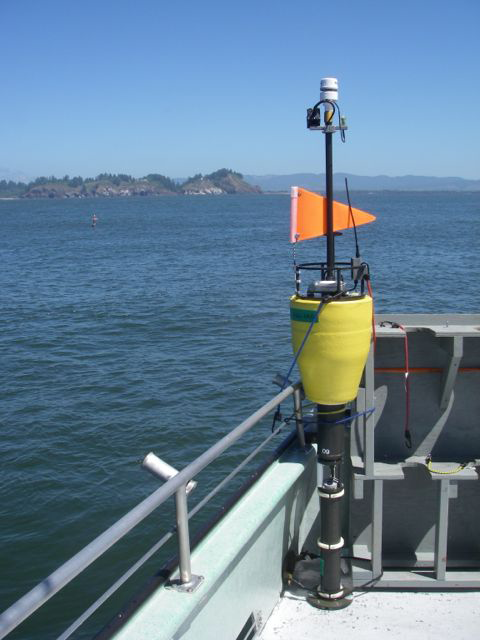
\includegraphics[width = 4cm,height=4cm]{swift_4.png}};
			\begin{scope}[x={(image.south east)},y={(image.north west)}]
				\draw[color=black, ultra thin,fill=white] (0.0,0.0) rectangle (0.21,0.16) node[pos=.5] {E};
			\end{scope}
		\end{tikzpicture}
		\label{fig:SWIFT}
	\end{subfigure}%
	\hfill
	\begin{subfigure}[b]{0.24\textwidth}
		\centering
		\begin{tikzpicture}
			\node[anchor=south west,inner sep=0] (image) at (0,0) { 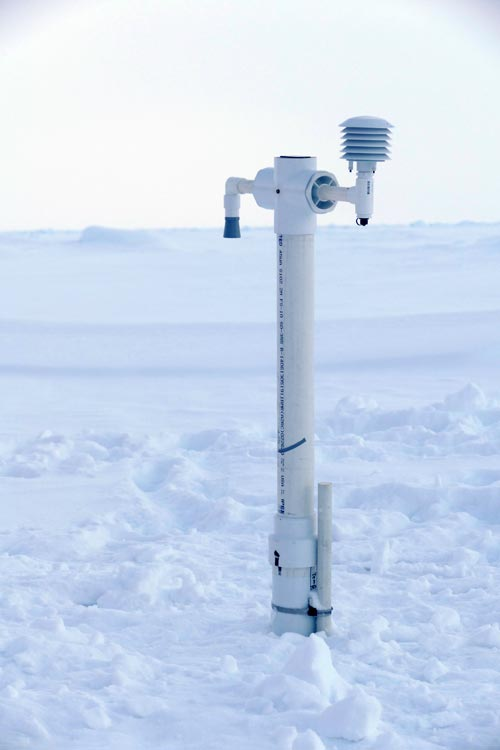
\includegraphics[width = 4cm,height=4cm]{SIMB.jpg}};
			\begin{scope}[x={(image.south east)},y={(image.north west)}]
				\draw[color=black, ultra thin,fill=white] (0.0,0.0) rectangle (0.21,0.16) node[pos=.5] {F};
			\end{scope}
		\end{tikzpicture}
		\label{fig:SIMB}
	\end{subfigure}%
	\hfill
	\begin{subfigure}[b]{0.24\textwidth}
		\centering
		\begin{tikzpicture}
			\node[anchor=south west,inner sep=0] (image) at (0,0) { 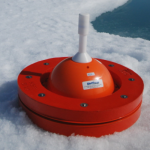
\includegraphics[width = 4cm,height=4cm]{UptempO.png}};
			\begin{scope}[x={(image.south east)},y={(image.north west)}]
				\draw[color=black, ultra thin,fill=white] (0.0,0.0) rectangle (0.21,0.16) node[pos=.5] {G};
			\end{scope}
		\end{tikzpicture}
		\label{fig:UptempO}
	\end{subfigure}%
	\hfill
	\begin{subfigure}[b]{0.24\textwidth}
		\centering
		\begin{tikzpicture}
			\node[anchor=south west,inner sep=0] (image) at (0,0) { 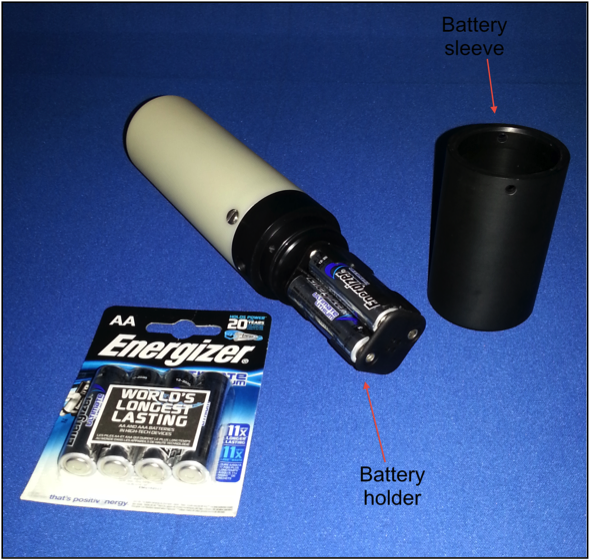
\includegraphics[width = 4cm,height=4cm]{trident.png}};
			\begin{scope}[x={(image.south east)},y={(image.north west)}]
				\draw[color=black, ultra thin,fill=white] (0.0,0.0) rectangle (0.21,0.16) node[pos=.5] {H};
			\end{scope}
		\end{tikzpicture}
		\label{fig:trident}
	\end{subfigure}%
	\hfill
	\caption{ Devices used for the comparison of autonomous instruments deployed in the sea ice region. Each device has been selected for its notability in published work as well as prevalence in sea ice and wave interactions in the Marginal Ice Zones. These devices are: (A) Wave in Ice Buoy developed by \textcite{rabault2017measurements} \cite{rabault2017measurements}, (B) Wave in Ice Observational System by \textcite{kohout2015device} \cite{kohout2015device}, (C) Novel Wave Directional buoys by \textcite{doble2017robust} \cite{doble_wave_2015}, (D) Surface Kinematic buoy by \textcite{guimaraes2018surface} \cite{guimaraes2018surface}, (E) Surface Wave Instrument Float Tracking buoy by \textcite{thomson2012wave}  \cite{jim_swift_2012}, (F) Seasonal Ice Mass Balance buoy by \textcite{polashenski2011seasonal} \cite{simbpic}, (G) Polar ISVP  by MetOcean \cite{uptempo}, (H) Trident buoy by Trident \cite{trident}.}
	\label{fig:buoys}
\end{figure}


A device that has sufficient autonomous and sustained capabilities will operate remotely with no human intervention. Therefore, the operating period of each device will be compared. This is the period between deployment and final transmission where the buoy is active. Additionally, the techniques for remote communication for each buoy will be examined in terms of data rates, coverage and transmission strategy to determine the techniques used to achieve remote communication effectively including a brief over view of available satellite networks. Then, to measure the sensing capabilities of each device, the measurement objectives of each device will be discussed as well as the hardware modules and software used to determine information. To compare the real time data collection, transfer and analysis, the device's processing strategy and storage strategies will be discussed. Data transfer techniques will be analysed with the remote communication section. Finally, device performance in the polar regions will be discussed through the success of each deployment, device deployment time, data integrity will be compared as well as devices that failed and the causes of those failures.

\begin{center}{\setlength{\extrarowheight}{5pt}%
		\begin{longtable}[H]{|>{\RaggedRight}m{0.3\textwidth}|>{\RaggedRight}m{0.2\textwidth}| >{\RaggedRight}m{0.4\textwidth}|}
			\caption{Devices used for the comparison including the device name, lead developer and the institution. These consist of both commercial and institutional devices for in-situ sea ice and wave measurements.}\\
			\hline
			\label{tab:device_list}
			\textbf{Device Name} & \textbf{Developed By} & \textbf{Institution}\\
			\hline
			Waves in Ice Buoy (WIIB) & Jean Rabault & University of Oslo, Norway \cite{rabault2019open} \\
			\hline
			Waves in Ice Observational System (WIIOS) & Alison Kohout & National Institute of Water and Atmospheric Research \cite{kohout2015device}, New Zealand \\
			\hline
			Novel Directional Wave Buoys (NDWB) & Martin J Doble &  Polar Scientific (Ltd.), United Kingdom \cite{doble2017robust}\\
			\hline
			Surface Kinematic Buoy (SKIB) & Pedro Veras Guimarães & Université de Bretagne Occidentale, France \cite{guimaraes2018surface} \\
			\hline
			Surface Wave Instrument Float with Tracking (SWIFT) Buoy & Jim Thompson & University of Washington Applied Physics Laboratory, United States of America \cite{thomson2012wave}\\
			\hline
			Seasonal Ice Mass Balance Buoy (SIMB) & Donald K. Perovich & Dartmouth College \\
			\hline
			Polar ISVP & MetOcean & MetOcean \\
			\hline
			UptempO & MetOcean & MetOcean \\
			\hline
			Trident Buoy & Trident Sensor & Trident Sensor \\
			\hline
		\end{longtable}
	}
\end{center}


\section{System Level Overview}

\subsection{Remote Communication}
\label{ch2:sec_remote}

On the Antarctic continent, remote communication is critical for ongoing scientific activities allowing for data to be transmitted from instruments to research stations and camps \cite{Sanghyun2016satellite}. These activities are further supported by high speed, high bandwidth communication networks such as fibre links \cite{jabbar2001multi} however, these networks have been implemented on a small scale to support permanent field camps \cite{Sanghyun2016satellite} on the continent. \textcite{Sanghyun2016satellite} show that communication from polar stations and field sensors to the rest of the world occurs using satellite constellation networks \cite{Sanghyun2016satellite}. These constellations are classified as  geostationary earth orbit such as Inmarsat \cite{inmarsat2021website} and Intelsat \cite{intelsat2021website} or low earth orbit (LEO) such as ORBCOMM \cite{orbcomm2021website}, Iridium \cite{iridium2019website}, Globalstar \cite{globalstar2021website} \cite{jabbar2001multi}. GEO satellites consist of 2 - 8 satellites orbiting the equator \cite{jabbar2001multi}. As a result, the network coverage is strong for mid-latitudes and weak for low latitudes. However, these satellites cover large areas providing longer connectivity (of up to 6.5 hours) \cite{Sanghyun2016satellite}. LEO satellites cover less surface area and have a smaller connectivity window (10 - 30 minutes). However, these constellations consist of more satellites. Additionally, the Iridium satellite network is the only LEO network that reaches the polar region \cite{jabbar2001multi} and allow for longer network connectivity. The constellation consists of 66 satellites \cite{Sanghyun2016satellite} and is well optimised for marine applications making it suitable for Southern Ocean sea ice applications. Iridium is a satellite network with global coverage and a variety of modems for various IoT uses. The company offers four main data services. Each service places constraints on the data transmission rates, bandwidth and modem selection. Each modem runs a data service that dictates the transmission rates, bandwidth and protocols.  Table \ref{tab:iridium service} shows the available network services. Furthermore, a full description of these modems is shown in table \ref{tab:ir_devices}. \par 

\begin{figure}[H]
	\centering
	\begin{subfigure}[b]{0.3\textwidth}
		\begin{tikzpicture}
			\node[anchor=south west,inner sep=0] (image) at (0,0) { 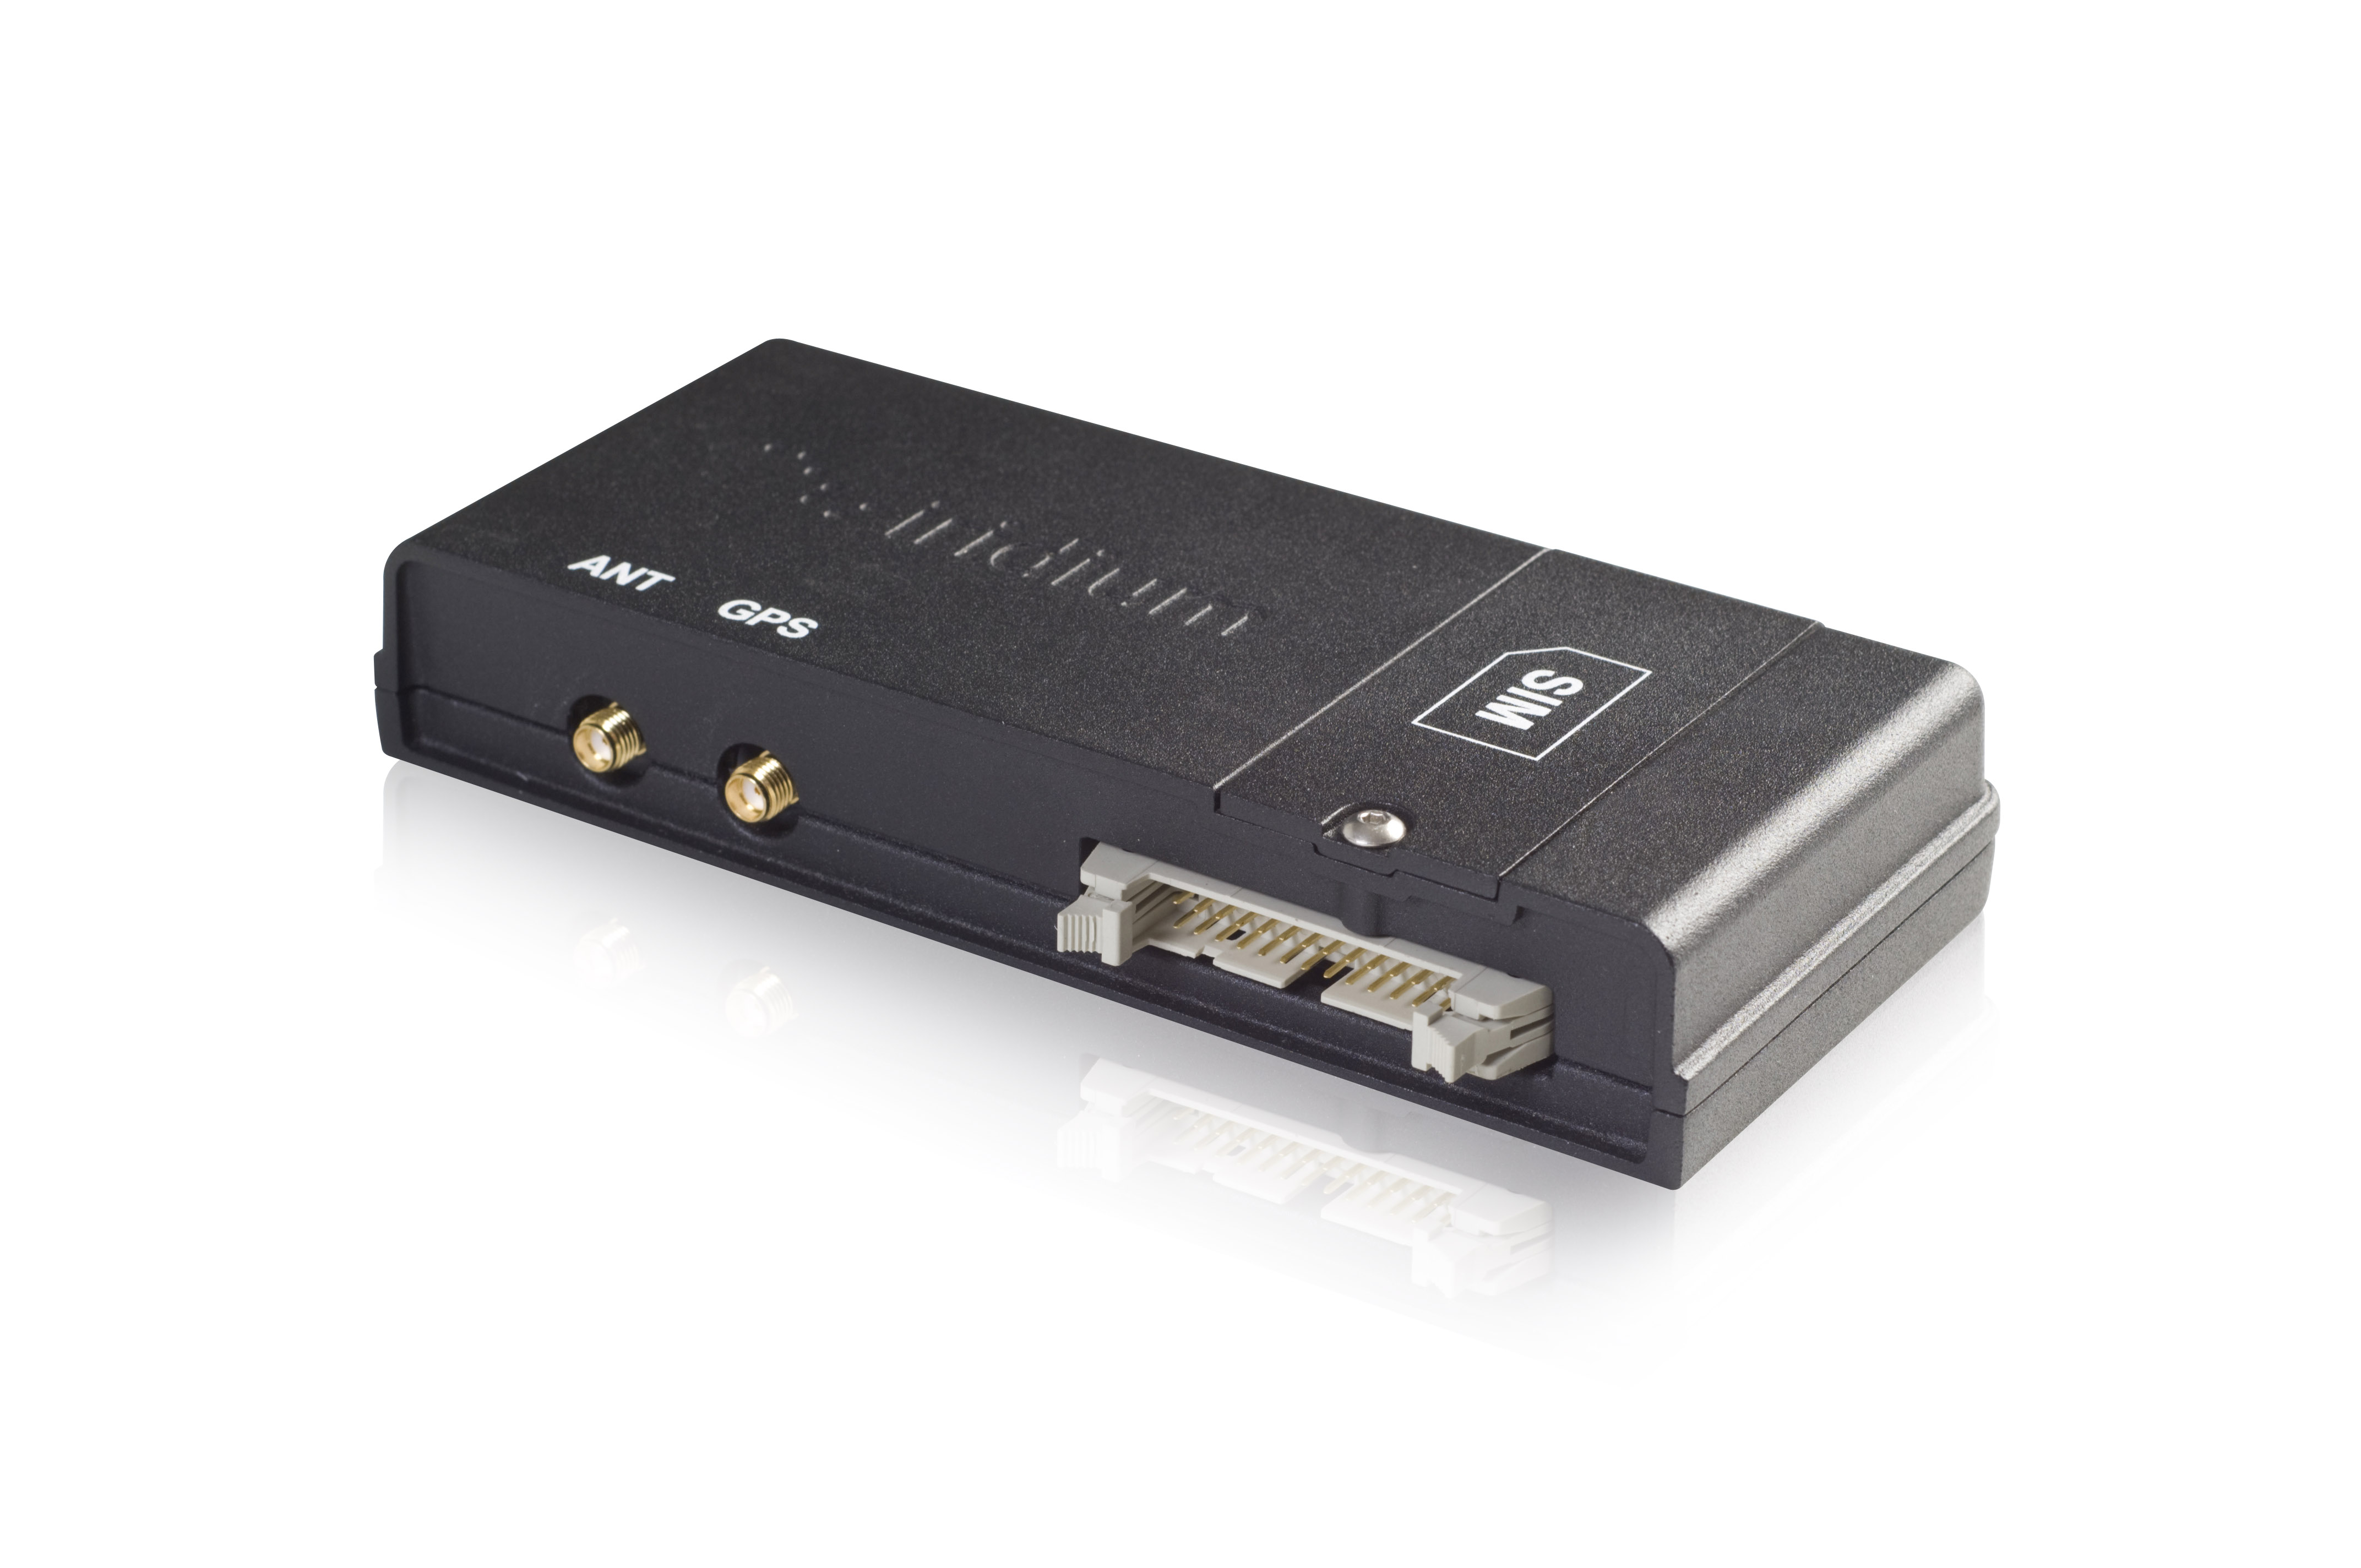
\includegraphics[width = 3cm,height=3cm]{9522B.png}};
			\begin{scope}[x={(image.south east)},y={(image.north west)}]
				\draw[color=black, ultra thin,fill=white] (0.0,0.0) rectangle (0.21,0.16) node[pos=.5] {A};
			\end{scope}
		\end{tikzpicture}
	\end{subfigure}%
	\hfill
	\begin{subfigure}[b]{0.3\textwidth}
		\begin{tikzpicture}
			\node[anchor=south west,inner sep=0] (image) at (0,0) { 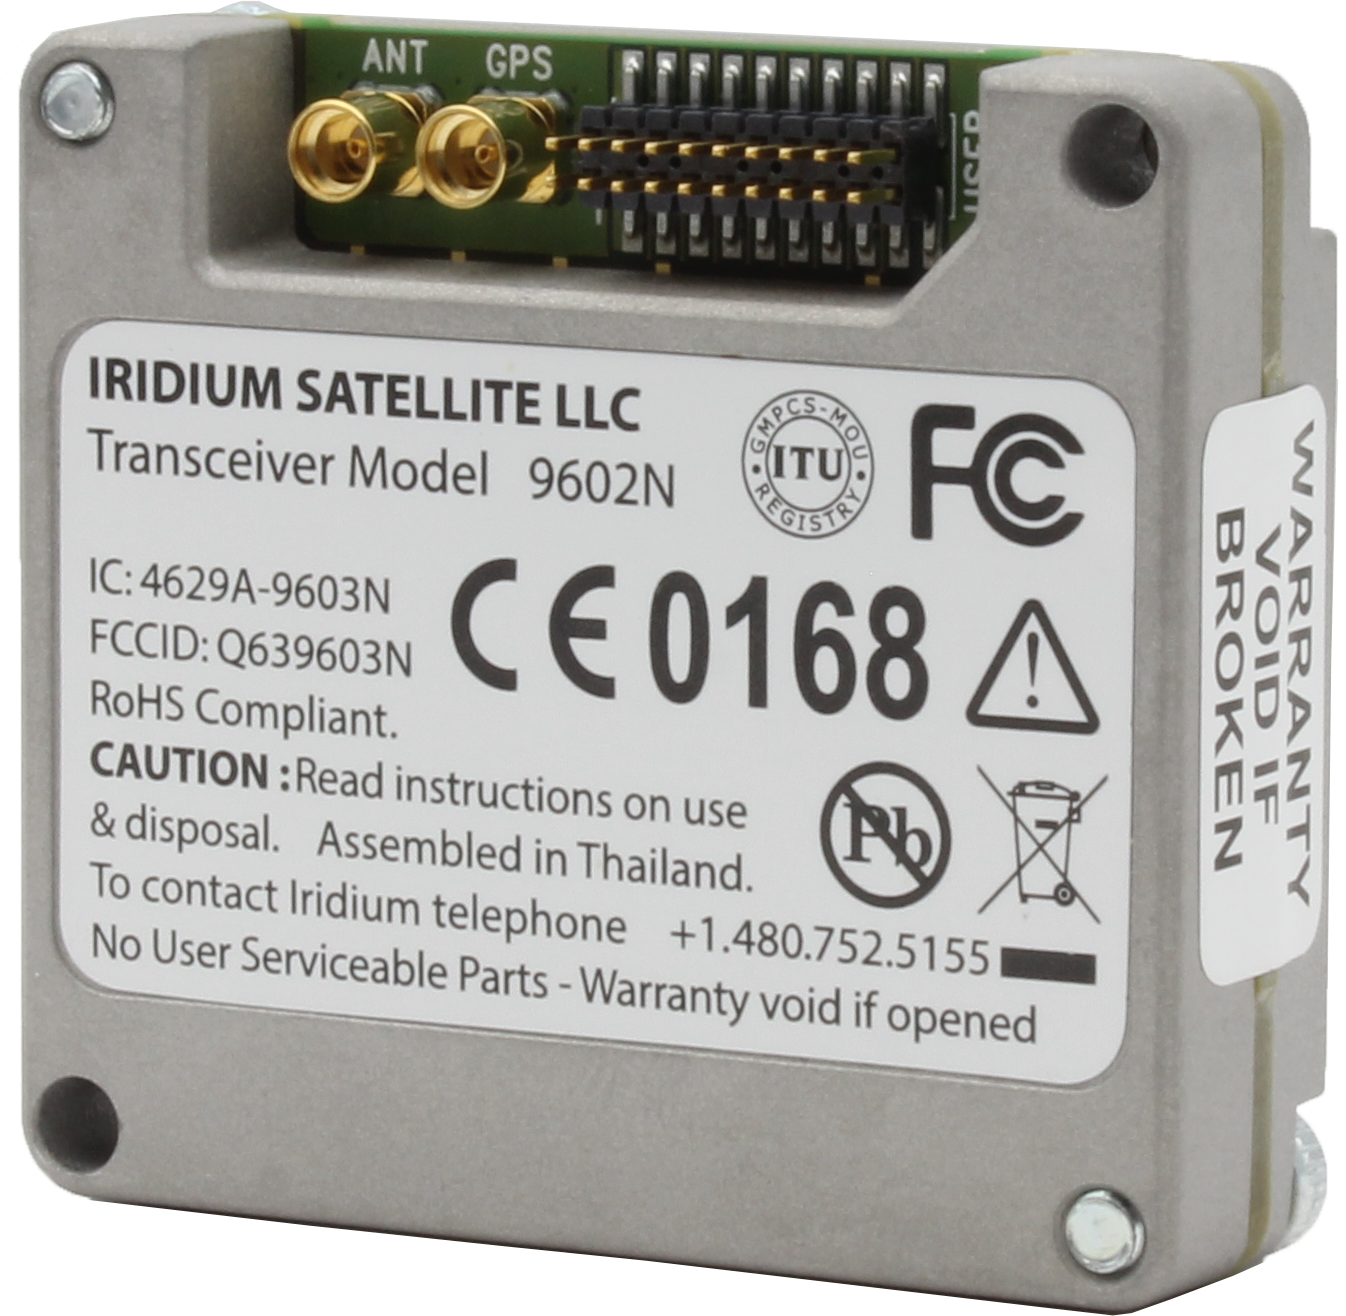
\includegraphics[width = 3cm,height=3cm]{9602.png}};
			\begin{scope}[x={(image.south east)},y={(image.north west)}]
				\draw[color=black, ultra thin,fill=white] (0.0,0.0) rectangle (0.21,0.16) node[pos=.5] {B};
			\end{scope}
		\end{tikzpicture}
	\end{subfigure}%
	\hfill
	\begin{subfigure}[b]{0.3\textwidth}
		\begin{tikzpicture}
			\node[anchor=south west,inner sep=0] (image) at (0,0) { 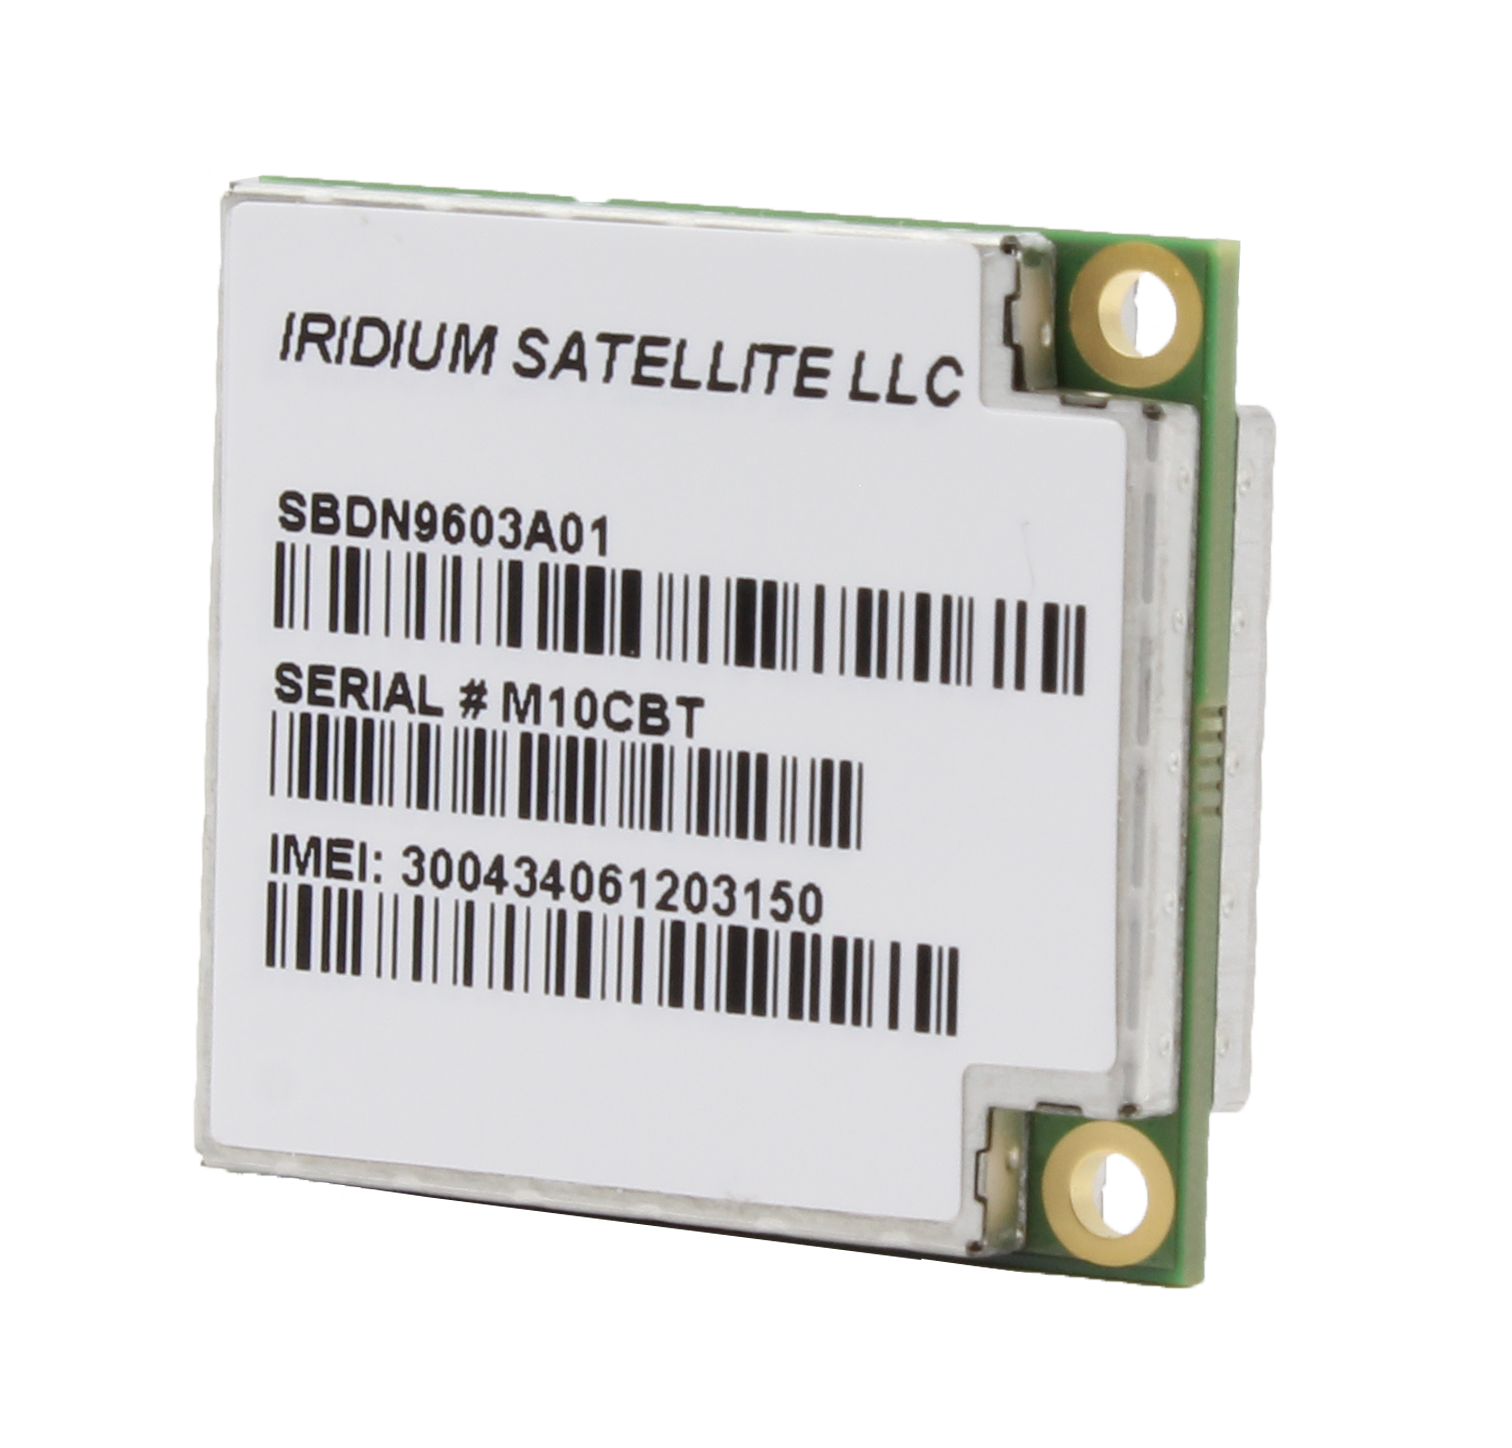
\includegraphics[width = 3cm,height=3cm]{9603.png}};
			\begin{scope}[x={(image.south east)},y={(image.north west)}]
				\draw[color=black, ultra thin,fill=white] (0.0,0.0) rectangle (0.21,0.16) node[pos=.5] {C};
			\end{scope}
		\end{tikzpicture}
	\end{subfigure}%
	\hfill
	\caption{Examples of popular iridium modems selected for remote communications. The 9522B modem (A) (image source: \cite{9522B}), 9602 modem (B) (image source: \cite{9602}) and 9603 modem (C) (image source: \cite{9603})} 
	\label{fig:irid_modem}
\end{figure}

Table \ref{tab:device_transmissionstrategies} shows the satelite network used by each device. All device use Iridium as the primary remote communication method. Other short range wireless systems such as Zigbee \cite{guimaraes2018surface} are alluded to however these systems are only used when the device is close by. Notably, The SIMB buoy details consideration for remote communication using the ARGOS satellite network however, the unreliability of the network resulted in irregular timestamped data \cite{planck2019evolution}. The network service, modem and transmission strategy of each device is shown in table \ref{tab:device_transmissionstrategies}.


\begin{table}[H]
	\centering
	\caption{ The following Iridium modems are compared in their key specifications. devices in the table were suitable for IoT applications based on prevalence in literature and recommendations from the manufacturer. Key parameters include weight, power consumption and transmission latency.Taken from \cite{iridium_product} }
	\label{tab:ir_devices}
	\resizebox{\textwidth}{!}{%
		\begin{tabular}{|l|c|c|c|c|c|}
			\hline
			\textbf{Device Name: } & \textbf{9602} & \textbf{9603} & \textbf{9522B\footnotemark} & \textbf{9523} & \textbf{Edge}\\
			\hline
			Weight (g) & 30 & 11.4 & 420 & 32 & 330 \\
			\hline
			Input Voltage (VDC) & 5 &5 & 4 -32 & 3.2-6 & 9 - 32V\\
			\hline
			Idle Current (mA) & 35 & 34 & 250 & 70 &300\\
			\hline
			Transmit Current (mA)& 140 & 145 &2.5$\times10^3$&500& 300 \\
			\hline
			Recieve Current (mA) & 40 & 39 &2.5$\times10^3$&110 & 300 \\
			\hline
			Packet Latency (s) &  20  &  20 & N/A &45 s& 20s\\
			\hline
			Price &	R2,526.07\footnotemark & 2,526.07\footnotemark & R23,317.40\footnotemark& R13,123.10\footnotemark & R5,638.18\footnotemark\\
			\hline
	\end{tabular}}
\end{table}
\footnotetext[2]{source: \url{https://www.rock7.com/shop-product-detail?productId=49}}
\footnotetext[3]{source: \url{https://www.rock7.com/shop-product-detail?productId=50}}
\footnotetext[4]{source: \url{https://satellitephonestore.com/catalog/sale/details/iridium-9522b-transceiver-496}}
\footnotetext[5]{source: \url{https://www.africasatellite.com/Iridium-9523-Core-Module-p/iridium-9523-core-module.htm}}
\footnotetext[6]{source: \url{https://www.rock7.com/shop-product-detail?productId=56}}

%figure of open-source buoy using the modem
Unanimously, all devices use the Iridium satellite network for remote communication with the Iridium 9602/3 SBD modem being used the most.  This choice is justified for its small form factor, low power and easy interfacing as shown in table \ref{tab:ir_devices} however it suffers greatly from limited bandwidth having a maximum transmission size of 340 bytes. Systems that use these modems for transmission of wave data rely on complex data processing algorithms and therefore do not transmit the raw time series. The only notable exception to this is the wave buoy developed by \textcite{doble2017robust} which continuously transmitted  data from an attitude and heading reference system (AHRS) as well as IMU time series data once every minute. For this purpose, they used the 9522B modem which allowed for continuous transmission using the RUDICS data service. This modem, along with the SBD modem used for the SWIFT Buoy also has a much larger SBD data buffer (1.92KB) However this device draws the most current during idle, transmit and receive states. Additionly this modem is expensive costing R23,317.40 compared to the 9523 (R13,123.10) and the 9602/3 (R2,526.07).  

\subsection{Power Supply}

A robust power supply is critical to support the functionality of a remotely deployed device. A successful power supply can extend the deployment range, duration, processing capabilities and functionality of sensors \cite{kennicutt2016delivering}. Device operation in the Southern Ocean MIZ presents a challenge where the constant freezing/ refreezing of the ocean surface layer prevents long-term infrastructure from being implemented. Hence, a remote device for sea ice monitoring requires a portable power source. Figure \ref{fig:powermoddiag} shows a diagram of a typical power module for a remote sensing device.

\begin{figure}[H]
	\centering
	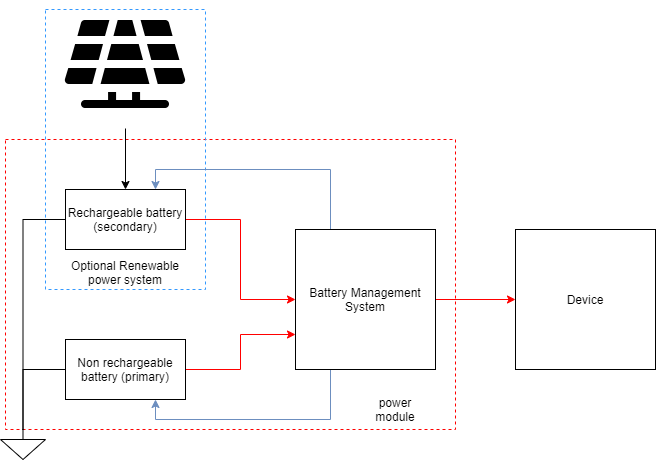
\includegraphics[width = 0.6\linewidth]{power module diagram.png}
	\caption{A block diagram of a typical power module for a remote sensing device based off the information from \cite{rabault2019open,doble2017robust,vidal2019xev}. Batteries are used as a primary source of energy which is connected to a battery management system to control and regulate the power supply to the device. optionally, solar panels are implemented with a rechargeable battery as a secondary power supply. Shown in the figure: flow of power (red), control lines (blue) and ground (black).}
	\label{fig:powermoddiag}
\end{figure}

Batteries such as lithium-ion are commonly used as sources of power for in situ devices. Batteries typically fall into one of two categories:
\begin{enumerate}
	\item Primary: Cells that cannot be recharged once they are depleted. These batteries have a high energy density and can store charge for long periods.\cite{besenhard2008handbook}
	\item Secondary: Cells that can be recharged. These cells are more cost effective with longer usage cycles \cite{besenhard2008handbook}.
\end{enumerate}

Lithium  Ion and Alkaline batteries are examples of primary cells that have commonly been used as they provide a cost effective solution due to their high energy density and long-term consistent life cycles \cite{zareer2018review}.  Secondary cells such as lead-acid, nickel-metal hydride and lithium polymer are commonly used coupled with a secondary charging circuit such as a solar panel \cite{manimekalai2013overview} to provide a more constant source of power. While batteries are cost effective solutions, the climate of the Southern ocean can affect the battery performance. Freezing air temperatures can reduce the capacity of a standard lithium cell by up to 50\% for temperatures below $-10^\circ C$ \cite{doble2017robust,ZHANG2003137}. Additionally, frozen batteries/ ice formation on batteries can stop them from working \cite{doble2017robust,manimekalai2013overview}.A solution to compensate for this reduction is to use rechargeable batteries coupled with a renewable power sources such as solar \cite{doble2017robust,rabault2019open}, wind and geothermal energy \cite{manimekalai2013overview}.Solar photovotaic (PV) cells is the fastest growing renewable energy source with the highest energy density \cite{jordehi2016parameter}. PVs have numerous advantages such as low maintenance and operational costs, wide temperature operations and long life-cycles \cite{jordehi2016parameter} which makes them ideal for long term operation in remote environments. However, the power output of PV cells are significantly affected by weather conditions \cite{sharma2015solar}. Therefore, areas with poor sunlight coverage will not benefit from solar panels. Additionally, power generation from solar panels is inconsistent and requires an additional storage bank capable of frequent charging and discharging. Wind energy can provide a viable alternative to solar energy. \textcite{vichi2019effects} show that the Southern Ocean hosts strong, consistent winds. However, the design and implementations have not been discussed in any of the literature. Therefore this options is provided as an area for future research. Finally, a critical component of the power system is a battery management system. This allows the power supply to opperate under safe conditions while meeting performance requiremnt \cite{vidal2019xev}. This module includes power monitoring, power control and energy cycle optimization. Table \ref{tab:device_power_source} below shows the power sources used by each device and the strategy used to manage it.
\begin{table}[H]
	\centering
	
	\caption{A comparison of power supply strategies of the different devices  showing the the power source, topology of the power supply module as well as the voltage supplied at the output of the module. Information that was unavailable at the time of research has been labeled as "Not reported"}
	\label{tab:device_power_source}
	
	\setlength{\extrarowheight}{5pt}%
	\resizebox{\textwidth}{!}{%
		\begin{tabular}{|>{\centering}m{3cm}|>{\raggedright\arraybackslash}m{4cm}|>{\raggedright\arraybackslash}m{4cm}|>{\raggedright\arraybackslash}m{4cm}|>{\raggedright\arraybackslash}m{4cm}|>{\centering\arraybackslash}m{3cm}|}
			\hline
			\textbf{Device Name} & \textbf{Primary Power Source} & \textbf{Secondary Power Source} & \textbf{Battery Management System} & \textbf{Output Regulation Strategy} & \textbf{Output Voltage} \\
			\hline
			WIIB & Lithium Iron Phosphate (LiFePO4) battery & None & ATMega328P for Power control & Boost Converter & 5V \\
			\hline
			WIIOS & Alkaline battery & None & Integrated into firmware & 8-cell series configuration, no regulator & 12V \\
			\hline
			NDWB & Alkaline battery & Solar panel and lead-acid battery & Not Reported & Not Reported & 12V \\
			\hline
			SKIB & Lithium thionyl chloride (LiSOCl2) battery & None & Not Reported & Not Reported & 3.6V \\
			\hline
			SWIFT & Alkaline or Lithium  battery& None & Not Reported & Not Reported & 14V \\
			\hline
			SIMB & Alkaline battery & None & Not Reported & LMZ12003 Step Down Converter (5V, 3.3V)\par MIC29201-12W Low dropout regulator (12V) & 3.3V \par 5V \par 12V\\
			\hline
			Polar ISVP & LiSOCl2 battery & None & Not Reported & Not Reported & 12V \\
			\hline
			Trident & Lithium cell battery & None & integrated into firmware & Low dropout regulator & 5V\\
			\hline
	\end{tabular}}
\end{table}
\footnotetext{Information available online at \url{https://github.com/jerabaul29/LoggerWavesInIce_InSituWithIridium/blob/master/ElectronicsList/list.md}}

Table \ref{tab:device_power_source} shows the power supply strategies of each device. All systems use primary batteries as a source of power with the most common choice being alkaline or lithium-based batteries. However, \textcite{doble2017robust} is the only exception where a secondary power source was adde consisting of a solar panel and lead-acid batteries. Systems deployed in the Arctic Marginal Ice Zone have been designed with a recharging system such as a solar panel in the case of WII Buoy and NDWB, however, most long-range deployment buoys have opted for non-rechargeable systems composed of Lithium Thionyl Chloride (LISOCL2) or Alkaline batteries. In the case of the high-power buoys (SIMB, WIIOS, NDWB, Polar ISVP) an array of 3.3V -3.7V cells is connected to provide a nominal voltage in series with a regulator to provide a stable output. The strategy for each system is to pack as many batteries in as possible to satisfy the long-term energy requirements \cite{doble2017robust,rabault2019open}. Finally, few devices have reported their battery management strategies. \textcite{rabault2019open} used an ATMega328P microcontroller as a power controller for their device which monitored the status of the battery. \textcite{trident} and \textcite{kohout2015device} however integrated power control into their main firmware allowing for them to control and monitor their power source off a single processor.

\subsection{Polar Performance}

This section outlines the deployment of the systems in the Arctic/Antarctic marginal ice zones and compares the survivability and performance of each system. The focus of this section will be predominantly on devices deployed in the marginal ice zone. Table \ref{tab:device_components} shows the significant deployment locations in the Arctic and Antarctic sea ice zones as well as the deployment objectives of each device. 

\begin{table}[H]
	\centering
	\caption{ comparison between the functionality and purpose of the buoy showing the critical measurements as well as the significant deployment locations either in the polar ice zones or in a location critical to the validation of the device.}
	\label{tab:device_deployment}
	\setlength{\extrarowheight}{5pt}
	\resizebox{\textwidth}{!}{
		\begin{tabular}{|l| >{\raggedright\arraybackslash}m{5cm}|>{\raggedright\arraybackslash}m{5.4cm}|>{\raggedright\arraybackslash}m{5cm}|}
			\hline
			\textbf{Device name} & \textbf{Deployment objectives} & \textbf{Antarctica Deployments} & \textbf{Arctic deployments}\\
			\hline
			\multirow{3}{*}{WIIB} & Wave energy attenuation &  Ross Sea landfast ice \cite{rabault2020development} &  Templefjord (Svalbard) landfast ice \cite{rabault2019open} \\
			& Significant wave height &  & Northeast Barents sea \cite{rabault2019open}\\
			& Data quality && \\
			\hline
			\multirow{5}{5cm}{WIIOS} &Ice drift&Ross sea marginal ice zone \cite{kohout_smith_roach_williams_montiel_williams_2020}&\multirow{5}{*}{-}\\ 
			& Waves in ice & Ross Sea packed ice zone \cite{kohout2015device} & \\ 
			& Ambient temperature & Weddel Sea marginal ice zone \cite{albarello2020drift}& \\
			& Atmospheric pressure && \\
			\hline
			\multirow{4}{*}{NDWB} & Ice drift  & \multirow{4}{*}{ - } & \multirow{4}{5cm}{Beaufort sea \cite{doble2017robust}} \\
			& Wave induced ice breaking &&\\
			& Ambient temperature &&\\
			& Atmospheric pressure &&\\
			\hline
			\multirow{2}{*}{SKIB} & Ice drift &\multirow{2}{*}{-} & North Atlantic ocean (France) \cite{guimaraes2018surface}\\
			& Surface waves &&\\
			\hline
			\multirow{6}{*}{SWIFT} & Surface images & Ross Sea \cite{ackley_2020_seaice} & Chukchi sea \cite{hosekova2020Attenuation} \\
			& Ocean waves & Weddel sea \cite{DeSanti2018OceanWave} &  Beaufort sea \cite{lund2018Arctic} \\
			& Turbulence profiles &&\\
			& Ocean current profiles &&\\
			& Conductivity && \\
			&Wind speed and direction && \\
			\hline
			\multirow{6}{*}{SIMB} & Surface and bottom ice position &Weddel sea \cite{hoppmann2015fmot} & Beaufort sea marginal ice zone \cite{PLANCK2019102792} \\
			& Snow depth& & \\
			& Atmospheric pressure&& \\
			& Ambient temperature &&\\
			& Vertical temperature profile& & \\
			& GPS Location&&\\
			\hline
			\multirow{3}{*}{Polar ISVP} & Sea ice drift & \multirow{3}{5.4cm}{Weddel Sea marginal ice zone \cite{deVos2021evaluating}} & \multirow{3}{5cm}{Western Arctic Ocean \cite{lei2020comparisons}}\\
			& Ambient temperature & &\\
			& Atmospheric pressure &&\\
			\hline
			\multirow{3}{*}{Trident} & Sea ice drift & \multirow{3}{5.4cm}{Weddel sea \cite{alberello2019drift}}
			& \multirow{3}{*}{-}\\
			& Ambient temperature & &\\
			& Battery voltage &&\\
			\hline
		\end{tabular}
	}
\end{table}

\textcite{kohout2015device} deployed five Wave in Ice Observational Systems (WIIOS) in the East Antarctic marginal ice zone during the Sea Ice Physics and Ecosystem Experiment (SIPEX) mission\footnote{1st deployment occured September 2012 \cite{kohout2015device}} with the goal of capturing wave in ice events with measurement goals shown in table \ref{tab:device_deployment}. Three devices were deployed by helicopters on ice floes while two devices were deployed via the ships crane. \textcite{kohout2015device}
note that deployment via crane was successful in spite of 7 m swell and 25 $m.s^{-1}$ winds. The device was fitted inside a Pelican box with a sealed membrane surrounded by a tyre for protection and flotation in case of melting \cite{kohout2015device}. Consequently, this places the buoy directly on the surface of the floe rendering it susceptible to snow build up and flooding as mentioned in the previous sections.  After deployment, the crew received 600 samples of data over 39 days in total. However, the first device failed 20 hours after deployment coinciding with the first large wave event captured the buoys \cite{kohout2015device}. The second large wave event resulted in the failure of two more systems just 9 days after deployment \cite{kohout2015device}. The fourth buoy lasted for 17.5 days. The final buoy survived the longest at 39 days. As a result only one device lasted for the expected time with the majority of data captured during calm events.

\begin{figure}[H]
	\centering
	\begin{subfigure}[b]{0.45\textwidth}
		\begin{tikzpicture}
			\node[anchor=south west,inner sep=0] (image) at (0,0) {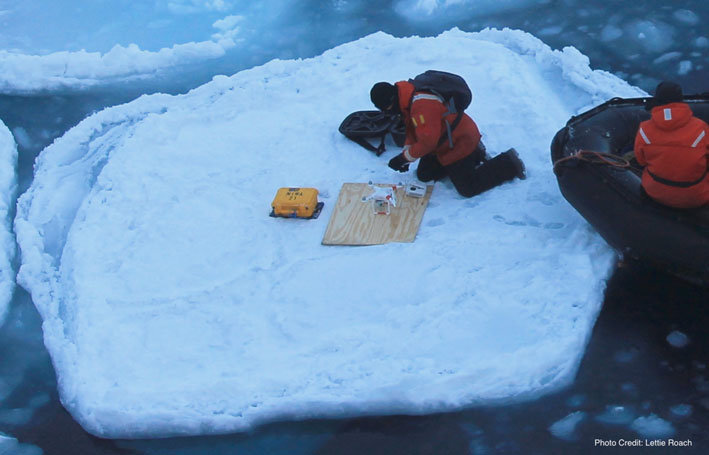
\includegraphics[width = 6cm,height=8cm]{WIIOS.png}};
			\begin{scope}[x={(image.south east)},y={(image.north west)}]
				\draw[color=black, ultra thin,fill=white] (0.0,0.0) rectangle (0.21,0.16) node[pos=.5] {A};
			\end{scope}
		\end{tikzpicture}
	\end{subfigure}%
	\hfill
	\begin{subfigure}[b]{0.45\textwidth}
		\begin{tikzpicture}
			\node[anchor=south west,inner sep=0] (image) at (0,0) { \includegraphics[width = 6cm,height=8cm]{Basket.jpg}};
			\begin{scope}[x={(image.south east)},y={(image.north west)}]
				\draw[color=black, ultra thin,fill=white] (0.0,0.0) rectangle (0.21,0.16) node[pos=.5] {B};
			\end{scope}
		\end{tikzpicture}    
	\end{subfigure}
	\caption{ Examples of different deployment protocols for ice tethered devices. In regions of consildated ice in favourable conditions, manned crews will step foot on the ice to deploy the device (A) (image source: \cite{kohout2020observation}), in unfavourable conditions, devices may deployed from a basket attached to a crane (B). A manned crew will lower the buoy on a suitable ice floe from the safety of the basket (image source: N. Taylor) }
	\label{fig:deploy}
\end{figure}
Two additional WIIOS buoys were deployed by \textcite{alberello2019drift} during the winter\footnote{first deployment occured in July 2017 \cite{alberello2019drift}}. Here, the buoys lasted significantly shorter than the previous deployment. The first system survived for 8 days while the second system survived for 3 weeks in spite of measures taken to place the device in power saving mode \cite{alberello2019drift}. This was achieved by lowering the sample period from to 2 hours. Consequently, the lower temporal resolution resulted in a significantly reduced accuracy of the ice deformation calculations \cite{alberello2019drift}. However, despite this low resolution, by operating at a temporal scale of 3 hours or less \cite{alberello2019drift}, one can effectively and accurately capture ice drift speed as well as the oscillations surrounding the movement. Additionally, \textcite{vichi2019effects} and \cite{albarello2020drift} discuss the deployment of two Wave in Ice Observation Systems similar to the ones by \cite{kohout2015device}. 2 devices were deployed on two separate ice floes 3 m in diameter and 100 km from the ice edge \cite{albarello2020drift}. One system survived for 8 days and 18 hours while sampling every 15 minutes before transmission ended \cite{albarello2020drift}. The second buoy however, survived for 6 days sampling every 15 minutes until it switched to power saving mode surviving for a total time frame of 3 weeks. \textcite{vichi2019effects} deployed a second pair of WIIOS buoys in a similar method to \cite{alberello2019drift} however, the first buoy stopped responding after 3 days while the second buoy survived for only 16 days \cite{vichi2019effects}. While the buoys survival is largely attributed to power optimisation, the lifespan could be influenced by the selection of the ice floe. Ice floe size and proximity to the ice edge affect the exposure of the floe to open-ocean processes and storms \cite{vichi2019effects}. This could result in failure due to ice mechanics which is discussed in section \ref{ch2:sec3_failiure}. \par 

\textcite{rabault2019open} deployed the waves in ice buoy (WIIB) WIIB on land-fast ice in the Ross sea \cite{rabault2020development} to test the device's performance in the Antarctic. In a similar fashion to the WIIOS buoy, the device was placed in a pelican case and attached to a flotation device, however, expected survival time for this device was significantly lower compared to the WIIOS devices: a maximum of 8 days \cite{rabault2019open} of continuous operation. The buoys by \textcite{kohout2015device} were designed to be expendable \cite{alberello2019drift} whereas the buoys by \textcite{rabault2019open} were designed to be retrievable. Additionally, the WIIB devices were deployed in the summer\footnote{First deployment date: December 2019 \cite{rabault2019open}}. Two devices were deployed in proximity however an ice break event resulted in the separation of the devices. The devices survived for 2.5 weeks \cite{rabault2019open} which \textcite{rabault2019open} attribute the failure to the devices having been crushed by ice and wave activity. Despite this, the devices were able to record significant wave events and maintain a fully charged battery throughout the deployment which \textcite{rabault2019open} attributes to the solar panel. 

\par \textcite{doble2017robust} alluded to a series of environmental considerations when designing the NDWB systems. One such consideration is the frosting over/ rimming of the device due to freezing ocean spray. Additionally, auxiliary power sources (i.e. solar panels) would need to account for long periods of no cloud cover \cite{doble2017robust}. Since the buoys were deployed by a manned crew, the design also had to account for ease of handling by the crew and not be too heavy \cite{doble2017robust}. The mechanical enclosure consisted of a float and a keel with the electronics contained above the surface in a dome. Twenty buoys were deployed in the Arctic marginal ice zone with each device anchored by drilling a hole in the ice and placing the keel inside. nineteen buoys survived the deployment with one system failing to boot. The buoys survived for extremely long periods with twelve systems surviving for two hundred days off a single alkaline battery pack \cite{doble2017robust}. A significantly longer period than both the WIIOS and WIIB systems. Seven systems ran for 70 days on alkaline batteries before switching over to  the solar powered lead-acid batteries. During this period, devices transmitted continuously over the Iridium network and were able to interpolate sea ice phases (see Section \ref{sec:ch1.section1}) from the tilt of the buoy \cite{doble2017robust}.

\subsubsection{Reasons for Failure}
\label{ch2:sec3_failiure}
\begin{figure}[H]
	\centering
	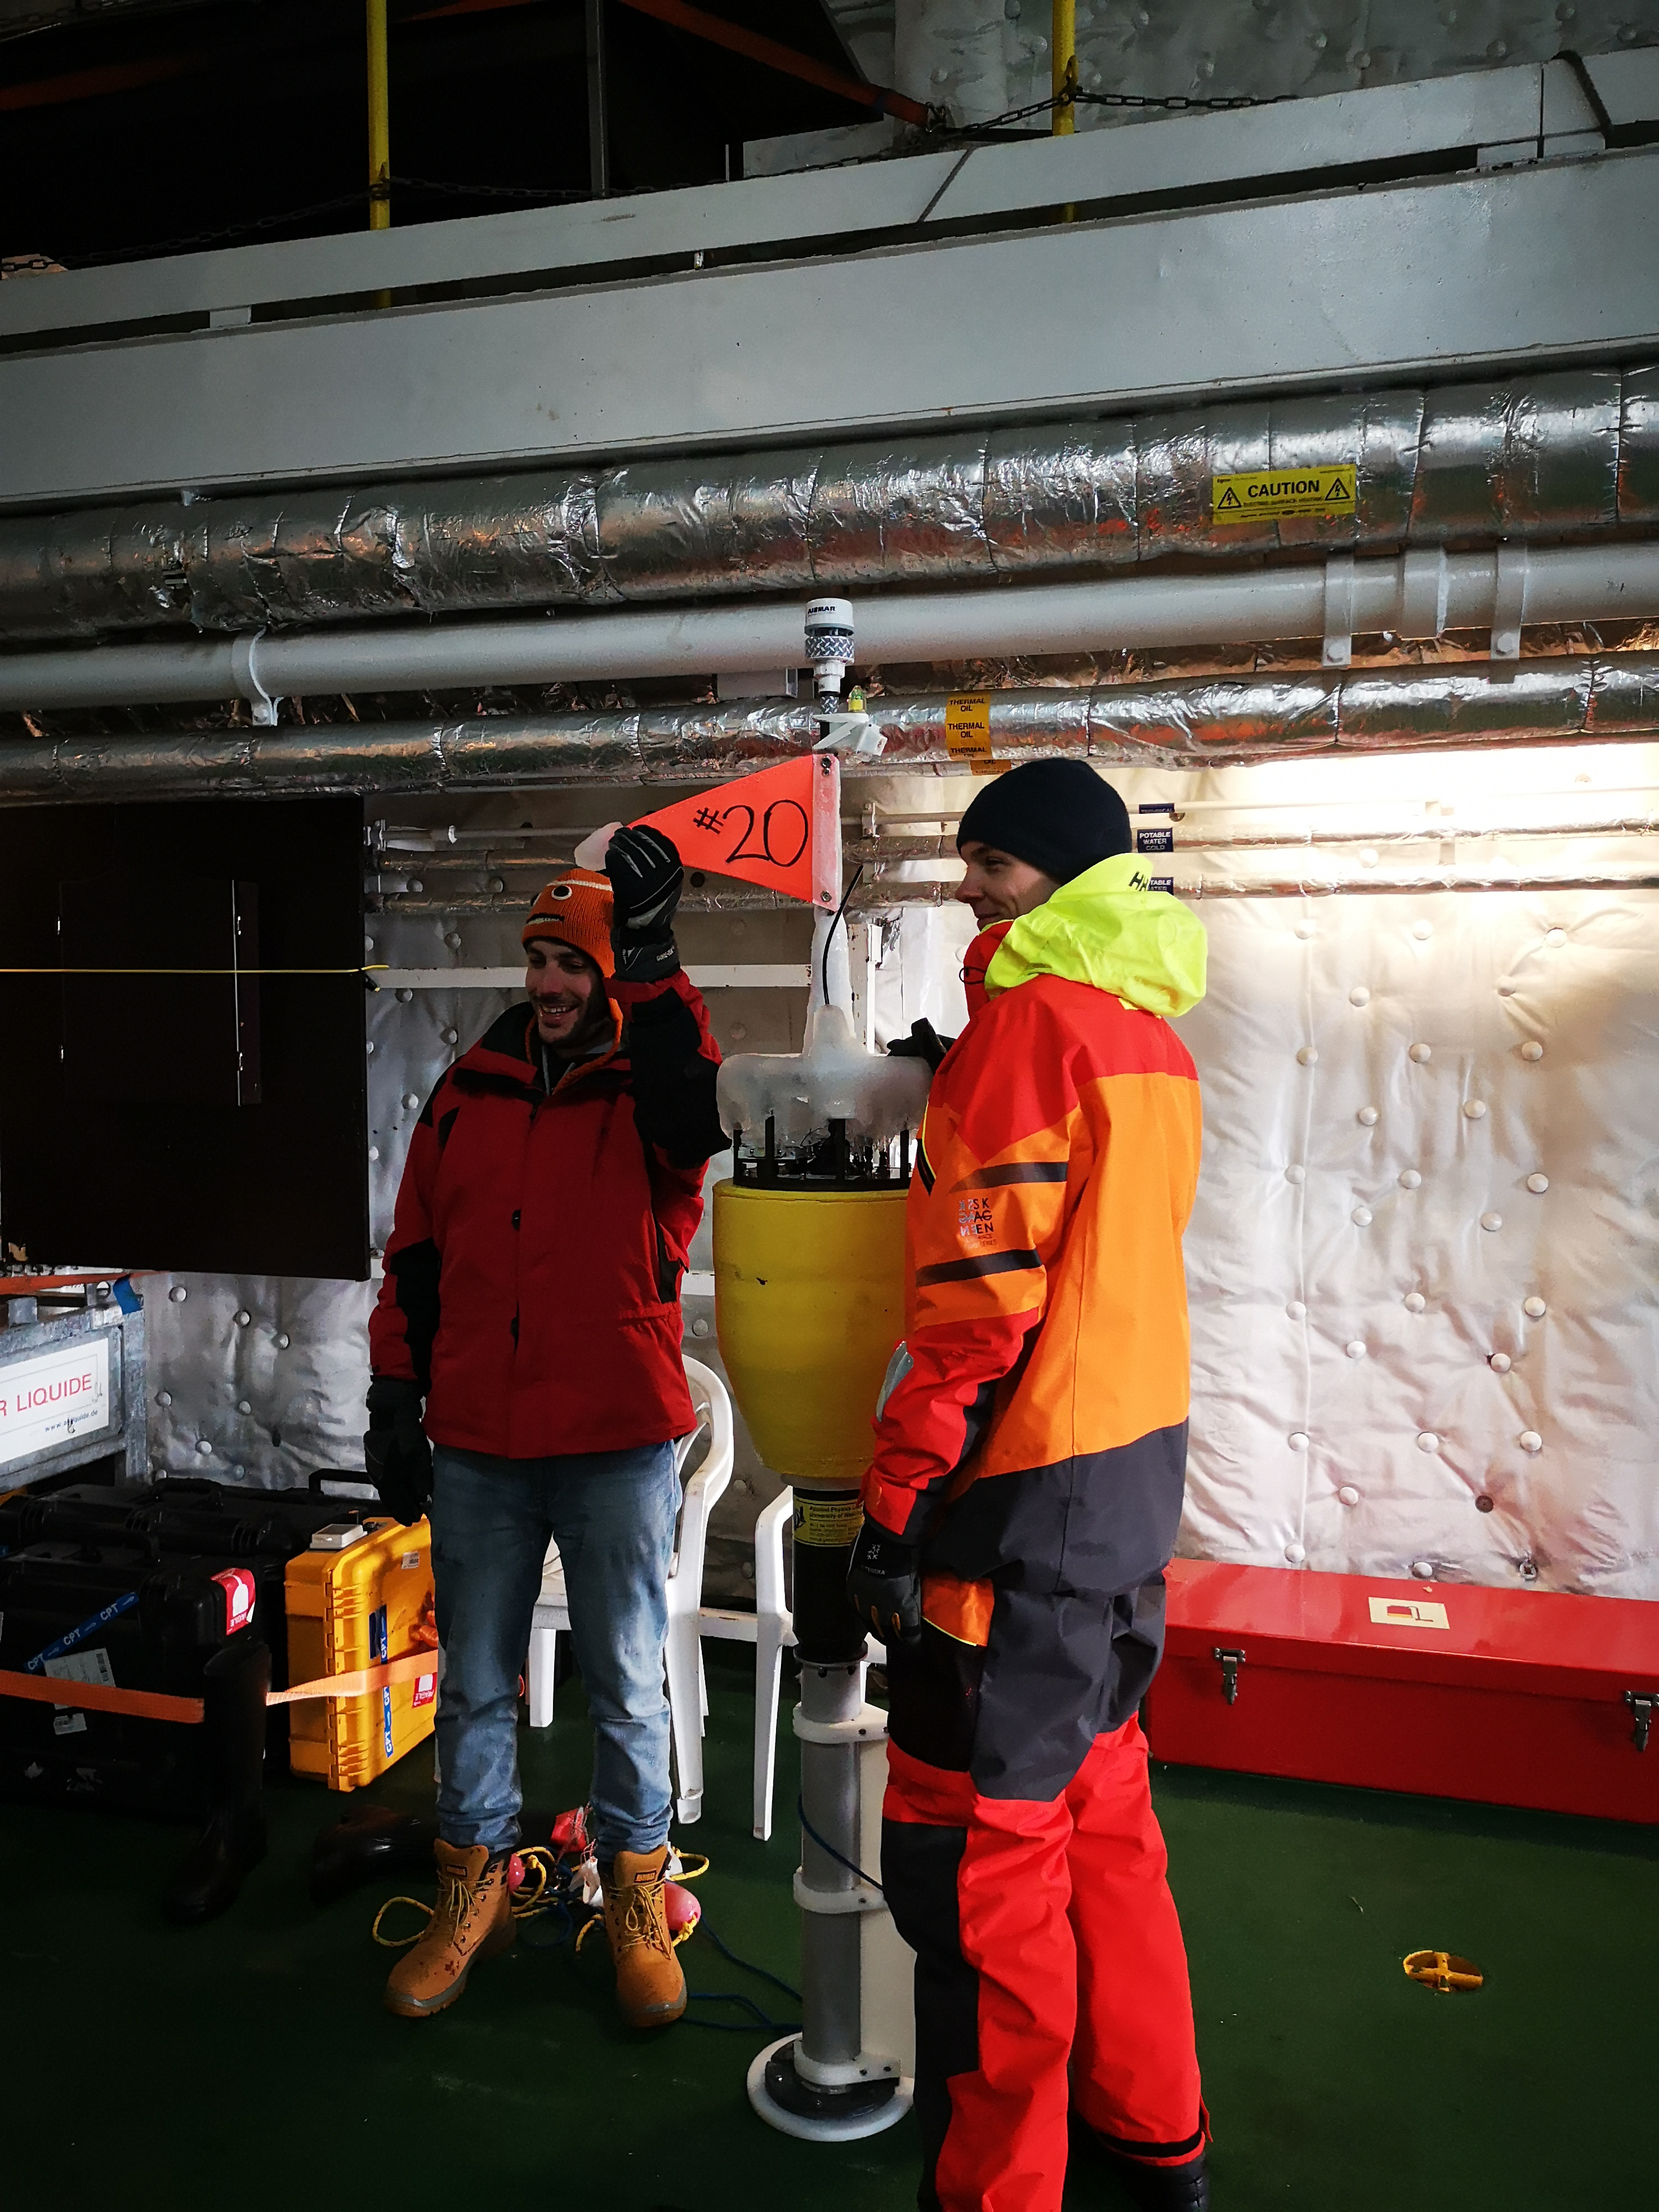
\includegraphics[width = 7cm]{swift_fail.jpg}
	\caption{During the 2019 SCALE winter expedition, a SWIFT device was retrieved early due to lost communication with the host. This failure was attributed to a build up of ice along the the rim from ocean spray. Photo taken by author.}
	\label{fig:swift_fail}
\end{figure}
Eventually, the systems by \textcite{doble2017robust} lost transmission 300 days after their deployment. This can be attributed to the depletion of the alkaline battery packs. The solar powered lead acid battery voltage eventually dropped below the alkaline battery voltage due to the lack of consistent solar coverage \cite{doble2017robust}. Additionally, sub zero temperatures have a tendency to reduce battery capacities by up to 50\% \cite{doble2017robust} however, \textcite{doble2017robust} found this estimate to be over conservative. Systems by \textcite{kohout2015device} and \textcite{doble2017robust} encountered similar failures with devices eventually depleting the on-board batteries. Additionally, \cite{alberello2019drift} attribute failiure of the first WIIOS system to the battery being depleted.\par 

Additional sources of failure experienced by \textcite{doble2017robust} include ice convergence. The systems were subject to ice-mechanics and as a result, ended up crushed by the floes due to rafting or buried under ice \textcite{doble2017robust}. These failures were identified when more than one system suddenly went offline. Devices also experienced freeze-over or were buried under snow which resulted in the devices going offline for temporary periods \cite{doble2017robust}. Additional evidence of rafting and ridging was captured by webcams on the buoy shortly before transmission ended \cite{doble2017robust}. Buoys that survived the spring melt refroze during the gradual refreezing of the ice. During the second cycle, none of the buoys rebooted when the ice melted in the spring \cite{doble2017robust}. Finally, the buoys developed by \textcite{kohout2015device} and \textcite{rabault2017measurements} sit in close proximity to the ice floes. As discussed previously, during the winter cycles, snow accumulates on the surface that can reach up to 1m in height. This snow formation can result in flooding where the floe becomes submerged. Prolonged burying under snow may have resulted in the device freezing over thereby losing contact while prolonged contact with the seawater may have resulted in the buoys failing on several occasions (\cite{kohout2015device,vichi2019effects,albarello2020drift,rabault2019open})\par 

Finally, \textcite{vichi2019effects} discuss the findings surrounding the failure of the first WIIOS system. \textcite{vichi2019effects} observed a major cyclonic event. The cyclone formed on  2 July 2017 and achieved lysis on 5 July 2017 which coincided with the buoy deployment. Following the event, four more cyclonic events were recorded with three explosive cyclones \cite{vichi2019effects} characterising a change of pressure over 24 hours. During this time, \textcite{vichi2019effects} observed winds speeds of up to $33$ $m/s^{-1}$ while noting that the air temperatures had increased to values "close to melting" \cite{vichi2019effects}. Additional observations found an increase in significant wave height in the activity. These conditions indicate deformation \cite{vichi2019effects} which may have subjected the buoys to forces experienced by \cite{doble2017robust} during their arctic deployment which were verified against the temperature and pressure readings of the second WIIOS during the cyclonic event. The buoys were deployed close to the ice edge exposed to greater open ocean processes and cyclonic activities than other semi-consolidated and consolidated regions \cite{vichi2019effects}. As a result, air advection, storms and large wave movement delay the consolidation of sea ice considerably \cite{vichi2019effects}. Hence, the ice floes were more likely to experience rafting, ridging \cite{icedefinition1992}, extended flooding, and freezing over which may have caused the failures of the WIIOS buoys.
\newpage
\section{Subsystem Overview}

This section focuses on the subsystem analysis and component selection for each system. As stated previously, each buoy was created with a unique objective shown in table \ref{tab:device_deployment}. These objectives have influenced the sensor selection, topology and layout of the overall subsystems. In addition, the device designs choices have been influnced objectives for developing new in situ technologies by \textcite{kennicutt2016delivering} as the device developers have factored in power consumption \cite{kohout2015device}, ease of use and deployment \cite{rabault2019open}, long-term operation \cite{doble2017robust},cost \cite{planck2019evolution,rabault2019open} and availability of infrastructure \cite{doble2017robust} over and above functionality. For example WIIB was developed using open-source hardware \cite{rabault2019open} in order to increase access to readily available technology while WIIOS was developed using off-the-shelf components \cite{kohout2015device} to create a cost effective device. From table \ref{tab:device_deployment} we saw that the principle measurements of each device share the following measurement objectives:

\begin{enumerate}
	\item Ice drift
	\item Wave data/Wave in Ice data
	\item Ambient temperature
	\item Atmospheric pressure 
\end{enumerate}

The following sections discuss how these objectives have influenced sensor selection for each of these measurements as well as the hardware, and software strategies implemented to achieve these objectives.

\subsection{Processing capabilities}

\begin{figure}[H]
	\centering
	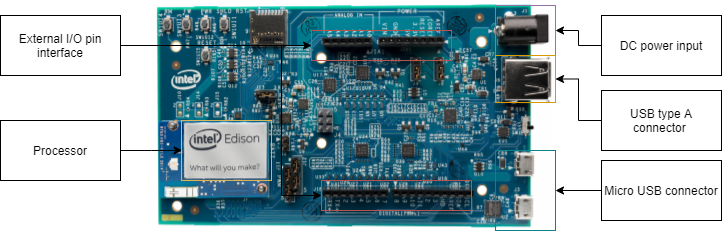
\includegraphics[width = 0.9\textwidth]{edison.png}
	\caption{Diagram of a typical microprocessor (yellow) on a development board. This device is an Intel Edison which was used as the main processor \textcite{kohout2015device} for the WIIOS. The development board allow for fast prototyping and integration into projects. The processor interface with external peripherals through physical input/output pins (Red) and contains standard serial communication ports such as USB (orange), micro USB (teal) and a connector for external voltage (purple). Image source: \cite{edison} }
\end{figure}
The processing capabilities of each device facilitate the functionality of each buoy. A strong processor allows for the implementation of in-situ data processing and wave analysis algorithms \cite{kohout2015device,rabault2019open}. Additionally, due to the bandwidth constraints mentioned in section \ref{ch2:sec_remote}, some devices require data compression algorithms to allow the data to fit in the transmission buffers. The functionality of these devices has been made possible through the use of microprocessors. These are programmable integrated circuits that contain processing elements \cite{subham2018micro} and form the basis of microcontrollers and microcomputers \cite{crisp2003introduction}. These components are small and are increasingly becoming integrated into affordable, widely available components such as Raspbery Pis and Arduinos \cite{rabault2019open}. The table below shows a comparison of processors and topological implemented in each design

\begin{table}[H]
	\centering
	\caption{Comparison of the processing strategy implemented by each device. Multiple processors have been used in a selection of devices hence included in the comparison is the number of processors used and the type of processor used as well as the function of each processor }
	\label{tab:device_process}
	\setlength{\extrarowheight}{5pt}
	\resizebox{\textwidth}{!}{%
		
		\begin{tabular}{|l|>{\centering\arraybackslash}m{3cm}|>{\raggedright\arraybackslash}m{5cm}|l|}
			\hline
			\textbf{Device name} & \textbf{Number of processors} & \textbf{Processor name} & \textbf{Function} \\
			\hline
			\multirow{3}{*}{WIIB}& \multirow{3}{*}{3} & ATMega 328P & Low power unit \\ \cline{3-4} & & Arduino Mega 2560 & Data Logger \\ \cline{3-4} && Raspberry Pi Zero & Wave processing \\
			\hline
			\multirow{2}{*}{WIIOS} & \multirow{2}{*}{2} & Intel Edison dual core & Wave processing \\ \cline{3-4}&& ATMega 328P & Low power unit \\
			\hline
			NDWB & 1 & ACME Systems Fox G20 & Power control \\
			\hline
			\multirow{2}{*}{SKIB} & \multirow{2}{*}{2} & EFM32-M3 & Wave spectral processing \\ \cline{3-4} && Unspecified processor & Power control \\
			\hline
			SWIFT & 1 & Sutron Xpert & Data processing \\
			\hline
			SIMB & 1 & ATSAMD21G18 & Data processing control \\
			\hline
			Polar ISVP & 1 & Global Platform Transceiver Controller (GPTII)\footnotemark[1] & Data processing and control \\
			\hline
			\multirow{2}{*}{Trident} & \multirow{2}{*}{2} & Unnamed microprocessor & Data processing \\ \cline{3-4} && Unnamed low power unit & power control \\
			\hline	
	\end{tabular}}
\end{table}

\footnotetext[1]{Developed by \textcite{uptempo}$^{\text{TM}}$}
From table \ref{tab:device_process}, we can see that each device has been developed either with a single, powerful processor or with multiple, low powered processors. NDWB for instance builds its system around the dominant sensor i.e. the AHRS IMU with a single processor controlling all the peripherals as well as allowing for data processing. Drift loggers such as Trident, and Polar ISVP feature sparser sets of electronics with smaller, lower-powered processors for power control and peripheral control, In contrast, WIIOS and WII Buoy compartmentalise subsystems with a cluster of processors handling different aspects from the buoy. This shows a focus on computation rather than sensing as multiple controllers are used to free the main processor for implementing advanced digital signal processing. SWIFT Buoy appears as the outlier as the system is built around a dedicated data logger i.e. The Sutron Xpert with an integrated processor and satellite communication link abstracting data processing strategies on the buoy side. The SIMB buoy has the most advanced and largest number of sensors of all the buoys. A commonality among the buoys is the use of off the shelf components and processors. Another predominant feature, the GPS is an Adafruit MTK339 as well as SAMD Chips, Raspberry Pis and Arduino boards whereas, for Trident and MetOcean, more expensive solutions are used. This shows that developers have opted for ready-made that components that are auxiliary to the main measurements. This should explain why some components on a system are more advanced than others.



\subsection{Measurement of Wave data using inertial measurement systems}

Typical wave state estimation are derived from calculating wave parameters such as significant wave height and dominant wave frequency \cite{williams2013wave}. Additionally, Wave data can be analyzed in terms of its power spectral density. The two main methods for wave data analysis presented in this section are the Kuik Method and the Welch-Earle Method. Further explanations can be found in Appendix \ref{kuik}. Both approaches rely on a discrete time series of inertial data from a device with 3 axes of acceleration of 3 axes of rotation \cite{kuik1988method,earle1996nondirectional}.

Devices that measure wave parameters such as significant wave height, wave spectra or ocean states, incorporate a sensor that measures the vertical acceleration and roll, pitch, and yaw in discretised space \cite{earle1996nondirectional}. These parameters can be measured using an accelerometer for axial acceleration and a gyroscope for rotational velocity \cite{fong2008methods}. These devices are typically integrated circuits manufactured using micro electro-mechanical systems (MEMS) and are often combined to form an inertial measurement unit (IMU) allowing for 6 axes of measurement from a single device \cite{fong2008methods}. IMUs can also be expanded to include a magnetometer which measures magnetic bearing in 3 axis\cite{ahmad2013reviews}.IMU selection is dependent on the following factors\footcite{ahmad2013reviews}:
\begin{enumerate}
	\item Package size
	\item Accuracy
	\item Response rate
	\item Degrees of freedom
\end{enumerate}

\begin{figure}[H]
	\centering
	\begin{subfigure}[t]{.3\textwidth}
		\begin{tikzpicture}
			\node[anchor=south west,inner sep=0] (image) at (0,0) { 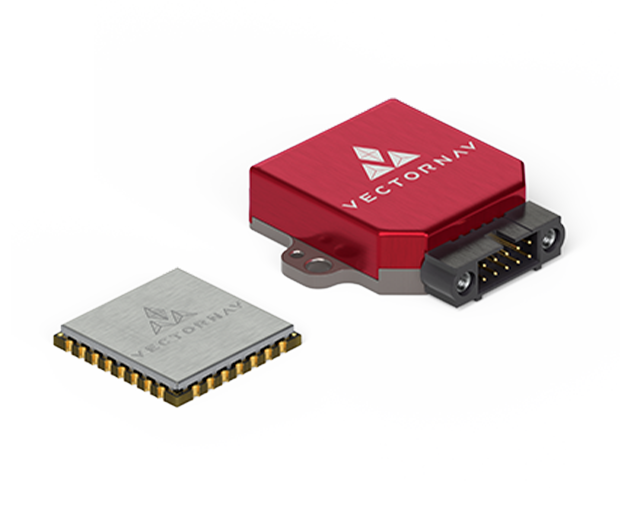
\includegraphics[width = 4cm, height = 6cm]{vn-100-smd-rugged_new.png}};
			\begin{scope}[x={(image.south east)},y={(image.north west)}]
				\draw[color=black, ultra thin,fill=white] (0.0,0.0) rectangle (0.21,0.16) node[pos=.5] {A};
			\end{scope}
		\end{tikzpicture}
	\end{subfigure}
	\hfill
	\begin{subfigure}[t]{.3\textwidth}
		\begin{tikzpicture}
			\node[anchor=south west,inner sep=0] (image) at (0,0) { 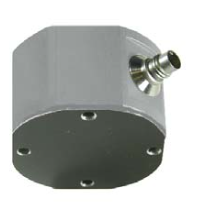
\includegraphics[width = 4cm, height = 6cm]{servokbeam.PNG}};
			\begin{scope}[x={(image.south east)},y={(image.north west)}]
				\draw[color=black, ultra thin,fill=white] (0.0,0.0) rectangle (0.21,0.16) node[pos=.5] {B};
			\end{scope}
		\end{tikzpicture}
	\end{subfigure}
	\hfill
	\begin{subfigure}[t]{.3\textwidth}
		\begin{tikzpicture}
			\node[anchor=south west,inner sep=0] (image) at (0,0) { 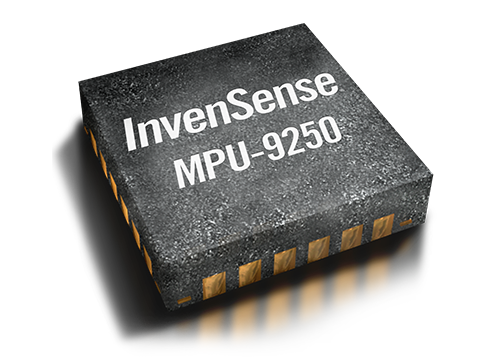
\includegraphics[width = 4cm, height = 6cm]{rp-mpu-9250.png}};
			\begin{scope}[x={(image.south east)},y={(image.north west)}]
				\draw[color=black, ultra thin,fill=white] (0.0,0.0) rectangle (0.21,0.16) node[pos=.5] {C};
			\end{scope}
		\end{tikzpicture}
	\end{subfigure}
	\hfill
	\label{fig:imus}
	\caption{Diagram showing examples of the different types of inertial measurement systems (IMUs) available for commercial use such as (A) an Attitude Heading Reference System (AHRS) VN100 \cite{vn-100} used by \cite{rabault2019open}, (B) an analog capacitive accelerometer 8330B3 Servo-Kbeam accelerometer used by \cite{kohout2015device} \cite{kistlerIMU} and (C) a 9 degree of freedom MPU9520 \cite{mpu9520} used by \cite{kohout2015device}. }
\end{figure}

\textcite{ahmad2013reviews} show that package size can limit the applications of the IMU. Additionally, IMUs require careful calibration and filtering in order to reduce the effects of bias offsets as well as low and high frequency drift \cite{fong2008methods}. More advanced filtering methods have been developed to improve the accuracy of IMUs such as Kalman filters \cite{simon2001kalman}  for positional estimates or Real-Time Kinetic Fusion (RTK) for velocity \textcite{meng2014optimal}. While important to the integrity of IMU data, these methods are usually implemented in software which is discussed in the upcoming sections. Finally, the degrees of freedom (DoF) influences the application of the IMU. The magnetometer is used to improve the accuracy of the gyroscope measurement and account for low frequency noise (drift) \cite{ahmad2013reviews}. However, removing the magnetometer is sensitive to magnetic distortion which can affect the measurements. \textcite{kohout2015device} encountered magnetic distortion during the SIPEX II deployments in September 2012 which rendered the magnetometer readings useless. In this section, the IMU is integral to deriving a time-series representation of inertia to calculate wave data as described above however, another application relevant to the literature is using IMUs to improve navigation \cite{ahmad2013reviews}. An IMU can be coupled with a Global Positioning System (GPS) device to determine position in areas with poor signal which can assist greatly with determine ice drift (discussed in section \ref{sec:ch2_drift}). Based on these considerations, table \ref{tab:imu_component} shows the IMU component selection for each device.
 
%TODO add table

\begin{table}[H]
	\centering
	\label{tab:imu_component}
	\setlength{\extrarowheight}{5pt};
	\caption{Comparison of the inertial measurement systems selected for each device showing the sensors included as well as the degrees of freedom.}
	\resizebox{\textwidth}{!}{%
		\begin{tabular}{|l|l|l|c|l}
			\cline{1-4}
			\textbf{Device name} & \textbf{Inertial Measurment Unit} & \textbf{Sensors} & \textbf{Degrees of freedom} &  \\ \cline{1-4}
			\multirow{3}{*}{WIIB} & \multirow{3}{*}{VN-100} & Accelerometer & \multirow{3}{*}{9} &  \\ \cline{3-3}
			&  & Gyroscope &  &  \\ \cline{3-3}
			&  & Magnetometer &  &  \\ \cline{1-4}
			\multirow{4}{*}{WIIOS} & 8330B3 Servo-KBeam & Vertical Acceleration & 1 &  \\ \cline{2-4}
			& \multirow{3}{*}{MPU9250} & Accelerometer & \multirow{3}{*}{9} &  \\ \cline{3-3}
			&  & Gyroscope &  &  \\ \cline{3-3}
			&  & Magnetometer &  &  \\ \cline{1-4}
			\multirow{3}{*}{NDWB} & \multirow{3}{*}{IG-500N} & Accelerometer & \multirow{3}{*}{9} &  \\ \cline{3-3}
			&  & Gyroscope &  &  \\ \cline{3-3}
			&  & Magnetometer &  &  \\ \cline{1-4}
			SKIB & LIS3DH & Accelerometer & 3 &  \\ \cline{1-4}
			\multirow{3}{*}{SIMB} & \multirow{3}{*}{BNO055} & Accelerometer & \multirow{3}{*}{9} &  \\ \cline{3-3}
			&  & Gyroscop &  &  \\ \cline{3-3}
			&  & Magnetomer &  &  \\ \cline{1-4}
			Polar ISVP & None & - & - &  \\ \cline{1-4}
			Trident & None & - & - &  \\ \cline{1-4}
		\end{tabular}
		}
\end{table}
As mentioned previously, systems such as WIIOS and WIIB have built their purpose around wave measurements and therefore have specified high powered, high accuracy IMUs for wave measurements. However, WIIOS buoy separates itself from WIIB by having a cheaper complimentary 9 dof IMU to complement the measurements \cite{kohout2015device}. SWIFT Buoy and the NDWB buoy use an integrated system known as an Inertial Navigation System (INS) with the former containing an SBG Elipse AHRS \cite{thomson2012wave} and the latter containing a IG-500-A1G2 \cite{doble2017robust}. This device contains a GPS and an Onboard processor for RTK fusion and Kalman filtering whereas other devices use an external processor for filtering. The SIMB Buoy is the only buoy on the list that has an IMU for non-wave related measurements. It uses a cheaper Bosch BNO055 which is used solely for measuring the orientation of the device.

\subsubsection{Software processing}

An IMU is a power device however extensive software proccessing is required to extract key parameters \cite{ahmad2013reviews}. Examples of software processing algorithms are shown in \textcite{kuik1988method} and \textcite{earle1996nondirectional}\footnote{See Appendix \ref{welchearl}.} for wave processing algorithms. Additionally, as mentioned previously, advanced filtering techniques are required to reduce the effects of low and high frequency noise. In this subsection the software processing strategy for each device given for extracting the desired parameters shown in table \ref{tab:device_deployment}.

\begin{table}[H]
	\centering
	\label{key}
	\caption{text}
	\setlength{\extrarowheight}{5pt}
	\resizebox{\textwidth}{!}{%
		% Please add the following required packages to your document preamble:
		% \usepackage{multirow}
		\begin{tabular}{|l|l|l|l|}
			\hline
			\textbf{Device name} & \textbf{Degree of Freedom used} & \textbf{Sample rate} & \textbf{Sample Period} \\ \hline
				\multirow{3}{*}{WIIB} & Vertical Acceleration & \multirow{3}{*}{10 Hz} & \multirow{3}{*}{25 minutes} \\ \cline{2-2}
				& Pitch &  &  \\ \cline{2-2}
				& Roll &  &  \\ \hline
				\multirow{4}{*}{WIIOS} & 3-axis acceleration & \multirow{4}{*}{2 Hz} & \multirow{4}{*}{11 minutes} \\ \cline{2-2}
				& 3-axis gyroscope &  &  \\ \cline{2-2}
				& 3-axis magnetometer &  &  \\ \cline{2-2}
				& Vertical  analog acceleration &  &  \\ \hline
				\multirow{5}{*}{NDWB} & 3-axis acceleration & \multirow{5}{*}{1 Hz} & \multirow{5}{*}{Continuous} \\ \cline{2-2}
				& 3-magnetometer &  &  \\ \cline{2-2}
				& heave &  &  \\ \cline{2-2}
				& roll &  &  \\ \cline{2-2}
				& pitch &  &  \\ \hline
				SKIB & 3-axis acceleration & 25 & 10 minutes \\ \hline
				\multirow{3}{*}{SWIFT} & 3-axis accleration & \multirow{3}{*}{5} & \multirow{3}{*}{9 minutes} \\ \cline{2-2}
				& Tilt &  &  \\ \cline{2-2}
				& Horizontal Rotation &  &  \\ \hline
				\multirow{2}{*}{SIMB} & Tilt & \multirow{2}{*}{-} & \multirow{2}{*}{-} \\ \cline{2-2}
				& Orientation &  &  \\ \hline
			\end{tabular}
	}
\end{table}
\par{WIIB}	

Raw Time series is passed through an Extended Kalman Filter running at 800Hz than a low pass filter. Wave Spectral data is calculated using the method by \textcite{earle1996nondirectional} where Co-Spectra is calculated using the Method by \textcite{kuik1988method}. Significant wave height is calculated through double integration. A Fast Fourier transform is applied to the data series to achieve this.
\par{WIIOS}

Data is filtered using a Butterworth filter with a cut-off frequency of 2Hz. Significant wave height is calculated by double integration using a Fast Fourier Transform. Spectra is calculated using the method by \textcite{earle1996nondirectional}.

\par{NDWB}

The double buoy is unique as it does not directly calculate wave parameters. However, the raw time series is filtered using an Extended Kalman Filter running at 10Hz

\par{SKIB}

Data collected from a sample window is processed using a classical RC filter to attenuate frequencies below 0.04Hz. \textcite{earle1996nondirectional} Spectra and Co-Spectra  Calculation is then applied.

\par{SWIFT}

The Swift buoy is the only device that uses multiple sensors for sea state calculation. First, data is collected more frequently in short intervals (9 minute sample periods every 12 minutes) which include Doppler Profiles, Camera images and IMU data. The INS System outputs a Real-time kinematic (RTK) fusion data series where IMU data is passed through a Coning \& Sculling Extended Kalman Filter running at 1KHz while the Doppler profiler is sampled at 8Hz. Turbulence profile is calculated through time-averaged data fitting of the Doppler profiler. The current state is calculated using the Stokes drift Equation over time-averaged velocity series. Finally, Wave information is calculated from an image of the sea state.

\par{SIMB}
No Clear Data processing strategy is available in the literature. This may be due to the non-critical nature of the IMU.

\subsection{Measurement of Ice drift using GPS}
\label{sec:ch2_drift}
The approach towards studying ice drift is typically performed using the techniques presented by \textcite{hibler1979dynamic} \footnote{See Numerical Modeling} where kinematic data is used to study ice drift dynamics and calibrate the ice drift model.\textcite{lepparanta2001sea} present two methods for data. The first method utilises measurement beacons are attached to the ice floes and used to track trajectories. The second method uses imaging devices such as radar, and satellites to determine ice displacement \cite{lepparanta2001sea}.\par

Each ice floe follows a unique trajectory \cite{lepparanta2001sea}  and individual trajectories combine to form a continuum. It has previously been believed that Sea Ice drift has been linked strongly to significant wave events \cite{alberello2019drift}. An experiment was conducted by \textcite{alberello2019drift} to measure the drift of sea ice during a cyclone event. Here it was found that wind velocity is the dominant driver of sea ice drift \cite{alberello2019drift} causing ice drifts of up to $0.75 m\cdot s^{-1}$ \cite{alberello2019drift}. Sea Ice drift speed is extremely sensitive to sampling rates. \cite{alberello2019drift} where sampling rates of 6 hours can underestimate the ice velocity by 5\% \cite{alberello2019drift} and up to 20\% for 12-hour sample rates. The consequence is reduced, near unusable, estimates of sea ice velocity components as well as drag coefficient and wind factor estimates. High temporal resolutions are capable of capturing important, inter-daily such as Ice oscillations. \textcite{alberello2019drift} state that to accurately capture Sea Ice behaviour, a temporal resolution of at least 3 hours is required \cite{alberello2019drift}. This not only allows for the capture of accurate drift speeds but provides an accurate characterization of Instantaneous velocities and Coriolis forces \cite{alberello2019drift}. Satellite observations OSI-SAF and METSAT are unsuitable for measurements hence a need arises for in -situ drift measurement devices. The GPS technology has been the standard for ice drift measurement. Current measurement sensing platforms such as those developed by \textcite{kohout2015device}, \textcite{rabault2019open}, \textcite{doble2017robust} and proprietary sensing technologies; Trident Buoy, SWIFT Buoy, Metocean. The GPS is set to measure data at relatively high temporal resolutions ranging from 15 minutes \cite{alberello2019drift} to 25 minutes \cite{rabault2019open}.

\subsubsection{Overview of GPS}

The principles that govern GPS have remained unchanged since its inception in 1973 \cite{spilker1996global}. The system consists of a satellite constellation that constantly broadcast their estimated position. A GPS device determines its position by matching a user-generated signal to that of 4 received satellites and comparing the phase difference to an on-board crystal oscillator \cite{spilker1996global}. This technique is called ranging and 4 satellites spread in a uniform geometry will allow for a device to calculate latitude, longitude, altitude and time to a relative degree of accuracy. The number of unknown signals correlates to the number of satellites required. Generally, a GPS device will have a lesser degree of accuracy than the satellites hence, an incoming signal can be used to correct the device's clock \footnote{provided altitude or time are already known \cite{spilker1996global}}.To accurately predict the satellite's trajectory, Satelite ranging is performed by a network of global monitoring which calculate the future position and send it back to the satellite. GPS signals are transmitted on two frequencies: 1575.42MHz and 1227.46MHz\cite{spilker1996global}. These are synchronously generated signals and allow a device to correct for ionospheric distortion. These bands carry modulated signals which are as follows: \cite{spilker1996global}


\begin{enumerate}
	\item Clear Acquisition Code:  This is a short code transmitted at 1.023 MHz and is used to request the Standard Positioning Service or SPS.
	\item Precise (P) Code: this is a much longer acquisition code. This signal is transmitted at 10.23MHz which is 10 x the rate of a CA code. This results in a much more accurate signal with less noise. This signal allows for the acquisition of Precise Positioning Service. However, this service is not available to unauthorized users and cannot be spoofed. As a result, this signal requires additional decryption.    
\end{enumerate}

\textcite{spilker1996global} also mention that military operators can degrade GPS signals which result in decreased accuracy from 20m up to 100m. The reduction of these accuracies requires differential GPS techniques, however, for the sake of this project. \par
once the acquisition signal is transmitted, the GPS device begins modulating at 50 bit/s. This allows the satellite to transmit its position as well as clock correction information to the device.\par
The GPS satellite constellation consists of 24 GPS satellites. These are configured into 3 rings of 8 satellites orbiting at different latitudes. The orbital altitudes were selected as 10.98 Nautical Miles \cite{spilker1996global}. This altitude was chosen to optimize user visibility with the number of crossings over United Sates ground stations, and cost of launching the satellites \cite{spilker1996global}. These satellites carry onboard atomic clocks for stability at $1\times10^{13}$ resolution. This allows for extremely accurate signalling as well as allowing for much more predictable time and position signals \cite{spilker1996global}. To achieve this, these atomic clocks are made out of either Cesium or Rubidium. Also, a frequency correction at $4.5\times10^{10}$ is provided to correct for relative shifts. \par
\subsubsection{GPS Error Modeling}
As mentioned before, the accuracy of the GPS signal is greatly affected by earth effects and satellite distribution. The main source of distortion is attributed to the earth's Ionosphere \cite{spilker1996global}. The ionospheric free electronics cause a delay in the modulated signal which is proportional to the sum of electrons along the signal's trajectory and inversely proportional to the signal's frequency squared. This delay is modelled as the product of a theoretical $90^\circ$ delay (Zenith delay) and a function of the elevation angle (obliquity factor). This results in a ratio of between 1.0 to 3.0 at small elevation angles \cite{spilker1996global}. This results in delays of 3m (often at night) to 20m (after midday). These delays are usually resolved by Satelite correlated positions. Correction can be performed in one of two ways:
\begin{enumerate}
	\item Transmission of Ionospheric model parameters as part of the message to the device and calculating the offset using that
	\item Using the two previously mentioned transmission frequencies directly measuring the delays in each broadcast frequency and estimating the position using the equation:\cite{spilker1996global}
	\begin{equation}
		1.546(delay_{L1} - delay_{L2})
	\end{equation}
\end{enumerate}

Navigation errors are characteristic of GPS performances. These errors are affected significantly by Satelite spread and ranging errors. Assuming the incoming signal is uncorrelated with a mean of zero, the RMS positional error is calculated as:
\begin{equation}
	RMS_{error} = (\text{Geometric Dilution})(\text{RMS Ranging errors})
\end{equation}

The geometric Dilution is modelled by estimating the precisional dilution of the spatial and temporal dimension measurements. This value estimates the quality of the GPS signal and is inversely proportional to the volume of the shape formed by 4 satellite \cite{jwo2001efficient}. Jwo (2001) outlines the procedure for the calculation of this value. Given a user's position on the earth, the distance from the user to the satellite is characterised by the equation:
\begin{equation}
	r =  s - u
\end{equation}
where $r$ is the distance from the user to the satellite, $s$ is the distance from the earth's centre to the satellite and u is the distance from the earth to the user. By measuring the propagation time from the user to the satellite, The absolute distance $||r||$ can be calculated and hence, the pseudo-range can be calculated as
\begin{equation}
	\rho_i = ||s_i-u||+ct_b + v_{\rho_i}
\end{equation}
where $\rho_i$ is the pseudorange for satelite i, c is the speed of light, $t_b$ is  the clock offset and $v_{\rho_i}$ is the noise of the pseudorange measurement and:
\begin{equation}
	||s_i-u|| = \sqrt{(x_i - x_u)^2+(y_i-y_u)^2+(z_i-z_u)^2} \text{ for } i \in 1,2,3...N \label{los}
\end{equation}
where N is the number of satelites and $(x_i,y_i,z_i)$ is the 3 dimensional position of satelite i. This represents a non-linear relationship for the line of sight of a satelite.  Jwo (2001) Explains that by creating a Taylor series centered on a nominal user position $(\hat{x_n},\hat{y_n},\hat{z_n})$ and ignoring the higher terms \cite{jwo2001efficient}. It then follows that:
\begin{equation}
	\Delta\rho_i = \rho_i - \hat{\rho_i} = e_{i1}\Delta x_u + e_{i2}\Delta x_u +  e_{i3}\Delta z_u
\end{equation}

The terms $e_{ij}$ represent the line of sight vector $E_i$ whereas the term $\hat{\rho_i}$ is the pseudo-range at the nominal user's position. It follows that the vector $E_i$ can be calculated as follows \cite{jwo2001efficient}.
\begin{subequations}
	\begin{align}
		e_{i1} = \frac{\hat{x_n} - x_i}{\hat{r_i}}\\
		e_{i2} = \frac{\hat{y_n} - y_i}{\hat{r_i}}\\
		e_{i3} = \frac{\hat{z_n} - z_i}{\hat{r_i}}\\
		\hat{r_i} = \sqrt{(\hat{x_n} - x_i)^2+(\hat{y_n} -y_i)^2+(\hat{z_n} -z_i)^2}
	\end{align}
\end{subequations}

Given n number of satellites, the equation \eqref{los} can be written as a matrix with the following form:
\begin{equation}
	\textbf{z} = \textbf{Hx}+ \textbf{v}
\end{equation}
\begin{equation}
	\Delta \rho _i = \begin{bmatrix}
		\Delta \rho_1 &  \Delta \rho_2 &  \Delta \rho_3 & ... & \Delta \rho_n
	\end{bmatrix} 
\end{equation}
where 
\begin{subequations}
	\begin{align}
		\textbf{H} = \begin{bmatrix}
			e_{11} & e_{12} & e_{13}& 1 \\
			e_{21} & e_{22} & e_{23}& 1 
			\\
			e_{31} & e_{32} & e_{33}& 1
			\\
			... & ... & ... &  1 
			\\
			e_{n1} & e_{n2} & e_{n3} & 1
		\end{bmatrix}\\
		\textbf{x} = \begin{bmatrix}
			\Delta x_u \\ \Delta y_u \\\Delta z_u \\ c\Delta t_b
		\end{bmatrix}\\
		\textbf{v} = \begin{bmatrix}
			v_{\rho_1}\\
			v_{\rho_2}\\
			v_{\rho_3}\\
			...\\
			v_{\rho_n}
		\end{bmatrix}
	\end{align}
\end{subequations}

The Matrix \textbf{H} is $n\times4$ where $n \geq 4$ to calculate all the paramters for GDOP \cite{jwo2001efficient}. We can then solve for the vector \textbf{x} by taking the psuedo inverse of H i.e $\hat{\textbf{x}} = (\textbf{H}^T\textbf{H})^{-1}\textbf{H}^t\textbf{z}$. Hence, given that the psuedo range is linearised, the quality of navigation is taken as the difference between the estimated position and the actual position \cite{jwo2001efficient}.
\begin{equation}
	\Tilde{\textbf{x}} = \hat{\textbf{x}} - x = (\textbf{H}^T\textbf{H})^{-1}\textbf{H}^Tv
\end{equation}
$E\{\Tilde{\textbf{x}}\Tilde{\textbf{x}}^T\}$ describes the covariance between the errors in the components of the estimated position \cite{jwo2001efficient} and is calculated as 
\begin{equation}
	E\{\Tilde{\textbf{x}}\Tilde{\textbf{x}}^T\} = (\textbf{H}^T\textbf{H})^{-1}\textbf{H}^TE\{\textbf{vv}^T\} (\textbf{H}^T\textbf{H})^{-1}\textbf{H}
\end{equation}
where $E\{\textbf{vv}^T\} = \sigma^2 I$. If all components of $\sigma$ are uncorrelated then the covariance becomes 
\begin{equation}
	E\{\Tilde{\textbf{x}}\Tilde{\textbf{x}}^T\} = \sigma^2(\textbf{H}^T\textbf{H})^{-1}
\end{equation}
and thus the GDOP factor can be calculated from the RMS values of $\sigma^2$ i.e.
\begin{equation}
	GDOP = \frac{\sqrt{\sigma_{xx}^2+\sigma_{yy}^2+ \sigma_{zz}^2+\sigma_{tt}^2}}{\sigma}
\end{equation} where $\sigma_{xx}^2$,$\sigma_{yy}^2$,$\sigma_{zz}^2$,$\sigma_{tt}^2$ are the RMS values of the x,y,z time components respectively. THe value GDOP can also be decomposed into the components PDOP,TDOP,HDOP,VDOP which represent the dilution of precision of Position, Time, Horizontal position and vertical position respectively.\par

Ranging errors are shown to come from 6 sources \cite{spilker1996global}:
\begin{enumerate}
	\item Satelite Ephemeris
	\item Satelite Clock
	\item Ionospheric group delay
	\item Trophospheric group delay
	\item Multipath scattering
	\item Hardware/software errors
\end{enumerate}




\subsection{Temperature Sensing and Measurement}

Environmental Sensing plays a pivotal role in predicting earth systemic processes. Tracking major events such as cyclones \cite{vichi2019effects} requires constant monitoring of antarctic environmental conditions. Temperature sensors can help predict atmospheric events such as storms, cyclones and seasonal changes as well as sea ice events such as sea ice melting \cite{kohout2015device} \cite{doble2017robust}. \textcite{doble2017robust} have discussed the significance of sea ice melting. This was considered a significant phase of sea ice and was classified as a phase in the development of their buoy. \par 

Temperature sensing technology is widely used for a variety of applications including food storage, mechanical failure warning systems, transport systems etc. \cite{awtrey2002environmental}. The majority of temperature sensing technology is used for thermal compensation as measurements such as pressure and humidity are dependant on environmental temperature \cite{mansoor2015silicon}. Thermal sensing technology exists in a variety of forms however, choice of sensor is heavily dependant on the application i.e. the object to be measured, the material state and the type of contact with the sensor \cite{mansoor2015silicon}\cite{childs2000review}. There are 3 main categories of measurement techniques \cite{childs2000review}:
\begin{enumerate}
	\item Invasive Measurements: Direct contact with an object of interest. This method is suitable for the measurement of objects in liquid or gas states. This category encompasses thermoelectric devices, liquid in glass thermometers, electronically resistive devices as well as semiconductor devices \cite{mansoor2015silicon}
	\item Semi-Invasive: Using the thermal measurement medium on an object and observing the effects of temperature such as thermal paints. Note: measurements are not directly taken from the object but rather the properties of the medium
	\item Non-Invasive: Object is measured from a distance using a device such as an infrared camera or acoustic thermography
\end{enumerate}
Also, the sensor selection must be based on the range, accuracy, resolution and precision of the device to ensure correct use An overview of different electric sensors is given below \cite{childs2000review}
\subsubsection{Thermocouples}

These devices use the principle of the Seebeck effect. Two conductors are joined at a junction which causes small electrons to flow \cite{pollock2017thermocouples}. This generates an EMF which is proportional to the temperature difference across their junctions \cite{pollock2017thermocouples}. Measurements are made using pairs of these conductors (referred to as thermo-elements \cite{pollock2017thermocouples}) one of the junctions is set to a known reference temperature (usually $0^\circ C$) while the other junction is measured. The resulting voltage is measured as a function of the temperature across the junction. In a practical sense, it may not be desirable to hold the reference voltage at $0^\circ C$, in this case, any reference voltage can be used provided it is fixed, repeatable and known \cite{pollock2017thermocouples}. a non-zero reference voltage will result in a relative voltage change. Hence this must be compensated in the measurement algorithm \cite{pollock2017thermocouples}. These devices have a wide temperature range from (-200 $^\circ C$ to 2000$^\circ C$ \cite{tong2001improving}). Despite this, there are some disadvantages. The temperature-voltage relationship is non-linear \cite{pollock2017thermocouples} \cite{tong2001improving} which can result in more intensive computational requirements as well as inaccuracies. Also, relative temperatures do not result in a stable voltage which gives uncertainty up to 2 $^\circ C$. Despite this, thermocouples are relatively cheap with a fast thermal response. However, this comes with a trade-off of increased noise. Finally, the temperature range of the thermocouple is limited by the metal used. Fortunately, thermocouples come in standard types \cite{tong2001improving} which have an associated range \cite{tong2001improving}
The relationship governing the emf and relative temperature change is shown to be. 
\begin{equation}
	E_{ab} = E_0 + a \Delta T+ b\Delta T^2
\end{equation}

$E_{ab}$ is the emf across the junction formed by conductors a and b. T is the measured temperature. $E_0$ is the reference temperature (a constant),  a and b are constants otherwise known as the relative Seebeck coefficients. These values can be determined by solving the above quadratic and are derived by Pollock (2017) as.
\begin{subequations}
	\begin{align}
		a = \alpha - \beta\\
		b = \frac{m_A-m_B}{2}
	\end{align}
\end{subequations}
$\alpha \text{ and } \beta$ are constants derived from the open circuit potential of conductors a and b respectively. $m_a\text{ and } m_b$ are the gradients of conductor and b respectively. \cite{pollock2017thermocouples}. 
\subsubsection{Resistive Temperature Detector}

Resistive Temperature Detectors (or RTDs) consist of metal with a known Temperature Coefficient. The device has a resistance that changes proportionally to the change in ambient temperature \cite{tong2001improving}. These devices are considered the most stable and accurate sensors \cite{tong2001improving} having an uncertainty range of $0.03^\circ C$ to $0.3^\circ C$ depending on the type. However, these sensors are considered more fragile and are largely expensive to obtain. These sensors come in the form of either a wound wire or a metal film with a known resistance at a specific temperature \cite{tong2001improving}. The advantage of these devices is a linear relationship between resistance and temperature. Hence a simple ohmic measurement \cite{tong2001improving} will allow for simple temperature prediction, however, these devices have a low sensitivity which can cause errors of up to $5 ^\circ C$ in this configuration \cite{tong2001improving}. A solution to this is to use four RTDs in a four-wire configuration where 2 wires provide excitement current and two wires connect to a voltmeter. This, however, adds to the complexity of the measurement and requires a more demanding processor. The measurements noise is proportional to the excitation current which causes the sensor to self-heat, According to Tong (2001) must be kept below 1mA to avoid significant noise distortion. Calibration of the sensor is performed against a compensation curve often provided with the device in question.
\subsubsection{Thermistors}

Modern Thermistors have progressed significantly in the past decade. Up until recently, they have been considered inaccurate with uncertainty ranges of up to 5\% \cite{tong2001improving}. Modern thermistors are capable of providing accuracies of up to 0.01$^\circ$. They consist of a semiconductor that changes its resistance in response to temperature \cite{childs2000review}. They have a faster response time than RTDs and work on the same principle for temperature measurement. However, where RTDs have a Positive temperature coefficient, Thermistors have a negative temperature coefficient \cite{tong2001improving}. These devices can operate over a substantial, albeit relatively limited, range of $-100^\circ - 300^\circ C$. The major trade-off with these devices is the lack of standards \cite{tong2001improving}. Operating the device involves a large degree of uncertainty. Also, these devices are not powerful enough to accurately reach the desired ranges alone. They need to be coupled with similar devices. Finally, the response curve is non-linear. The  relationship between resistance and temperature is \cite{childs2000review}:
\begin{equation}
	R_T = R_0e^{1 - B(\frac{1}{T}- \frac{1}{T_0})}
\end{equation}
where $R_T$ is the temperature measured, $R_0$ is the resistance at a known temperature $T_0$, T is the temperature and B is a coefficient based on the properties of the thermistor. Finally, these devices are more prone to noise from excitation current.
\subsubsection{Silicon Temperature Devices}

Semiconductor temperature devices are suited to applications where the temperature ranges from -55 to 150 $^\circ C$ these devices are capable of providing a stable output with a typical accuracy of $0.8 ^\circ C$. These devices typically consist of diodes and transistors with a bandgap voltage that changes with a change in temperature \cite{childs2000review}. These devices are advantageous in electronic application due to their small form, high accuracy and stability. These devices are relatively simple and have a good sensitivity to changes \cite{childs2000review}. Diodes are typically used in semiconductor devices. Here, the forward voltage drop across the p-n junction is linearly proportional to the Ambient temperature over a certain temperature range (typically 25K - 400k) \cite{childs2000review}. These devices are made out of either silicon or Galium-Arsenide. Silicon is preferred as it has better stability at low temperatures and is cheaper however, this comes at the trade-off of a lower voltage output \cite{childs2000review}. \par These Types of devices are readily available in IC forms and are manufactured in a variety of packages, types and compositions for any application. Typical devices are DS18B20, LM355 or BMP2080. Recent innovations in Silicon sensing have seen the rise of CMOS devices and Micro Electrical-MEchanical Systems (MEMs) being used more frequently \cite{mansoor2015silicon}. While these devices can suffer from deterioration due to self-heating, \textcite{mansoor2015silicon} discuss that the low-power operation of these devices can offset this issue. This is advantageous for systems that are constrained by power consumption. However, a major disadvantage with these devices is that these devices work ideally with a purely DC signal.An AC coupled signal can cause significant errors in the output \cite{childs2000review} \cite{mansoor2015silicon}. These errors can be the result of improper shielding and poor grounding. Hence proper shielding and grounding are required to reduce these errors. Finally, these devices require careful calibration before use.

\subsection{Atmospheric Pressure Sensing and Sensors}
Atmospheric pressure is a key measurement for environmental sensing. There has been an increased demand for in-situ environmental monitoring as mentioned by \cite{vichi2019effects} \cite{kennicutt2014polar} \cite{kennicutt2016delivering} \cite{kennicutt2019sustained} \cite{alberello2019drift}. It can provide insight into wind currents and storm events as well as predict trajectories of these storms. Also, pressure characterises the relationship between Atmospheric and ocean air process. The pressure is a Temperature dependant measurement \cite{mansoor2015silicon} and, often, Autonomous platforms couple pressure sensors with temperature sensors on the same Integrated Circuit (IC). One example is the BMP280 environmental sensor developed by Bosch \footnote{More details provided by Bosch Sensortech }. The current state of Pressure Sensing technology is driven towards Miniature MEMs version of large scale devices \cite{eaton1997micromachined}. Most large scale pressure sensors consist of a diaphragm mounted on a device in a known way. The diaphragm is coupled to a device that converts the pressure to a mechanical movement which is then measured using a gauge. These senses often had a secondary sensor that would convert the mechanical movement to an electrical signal which was then measured \cite{eaton1997micromachined}. Other sensors include barometers, bourdon tubes and vacuum pressure gauges. Most MEMs are based on these principles.\par 
\textcite{eaton1997micromachined} discuss the importance of micro-machined pressure sensors and provide an overview of various sensors. These can be classified as piezoresistive, capacitive, optical and resonant each with their pressure relationship.
\subsubsection{Diaphragm Based Sensors}
Previously mentioned, Diaphragm sensors determine pressure by measuring the deflection of a miniature diaphragm. This deflection is converted to an electrical signal. Typically, a reference pressure is provided as a measurement of a sealed chamber or absolute pressure port. Assuming the simplest version of this sensor i.e. a plate of uniform thickness \cite{eaton1997micromachined} The deflection $w$ of the diaphragm is related to the pressure  $P$ by the following equation: \cite{eaton1997micromachined}

\begin{equation}
	w(r) = \frac{Pa^4}{64D}(1- (\frac{r}{a})^2)^2
\end{equation}

where r is the deformed radius of the diaphragm, a is the original radius and D is the  rigidity of the diaphragm governed by the equation:

\begin{equation}
	D = \frac{Eh^3}{12(1-v^2)}
\end{equation}
where E,h,v are Young's modulus, thickness and Poisson's ratio of the disc \cite{eaton1997micromachined}. This technique suffers from a multitude of problems namely, the diaphragm is susceptible to plastic deformation and more robust diaphragms result in more complex relationships. The current relationship is nonlinear and can result in calculation errors. Eaten (1997) advocate for the use of MEMs based electronics on these principles.
\subsubsection{Piezoresistive Sensors}

Piezoresistive sensors are electric devices constructed out of a semiconductor whose electrical properties change when a stress is applied \cite{eaton1997micromachined}. these devices are mounted to a diaphragm and exhibit a linear change in resistance with a change in Pressure. Currently, these sensors take the form of single-crystal diaphragms with piezoelectric resistors diffused through the materials. The advantage of these devices is robustness towards hysteresis and measurement drift. At low temperatures, silicon exhibits near-perfect elastic behaviour and is  3 times the tensile strength of strain gauges\cite{eaton1997micromachined}. The sensors are, however susceptible to thermal expansion and can exhibit significant temperature drift \cite{samaun1971ic}. Additionally, these sensors require resistors with identical temperature Resistance characteristics otherwise the measurements will be inaccurate. Finally, additional compensation techniques are required.

\subsubsection{capacitive sensors}

These sensors consist of parallel conductive plates. Assuming a constant, known dielectric, an external pressure causes the plates to deform which changes the capacitance C according to the relationship \cite{eaton1997micromachined}
\begin{equation}
	C = \int \int \frac{\epsilon}{d - w(r)}drd\theta
\end{equation}

where $w(r)$ is the deformation of the plate, $\epsilon$ is the strain experienced on the plate and d is the distance of separation. The Pressure capacitance relationship can be approximated using a least-squares fit \cite{eaton1997micromachined} however this results in model errors of 1.5\% and up to 11\% at $w = \frac{1}{2}h$ the height of the plate. These sensors are more advantageous over piezoresistive sensors as they have higher pressure sensitivity and reduced susceptibility to temperature drift. However, these sensors are significantly susceptible to parasitic capacitance which can result in losses and errors. Additionally, these sensors are simple in design however they tend towards more complex circuit requirements.

